\documentclass[11pt]{article}

\usepackage[bookmarks=true,bookmarksopen=true]{hyperref}
\usepackage{url}
\usepackage{datetime}
\usepackage{proof}
\usepackage{enumerate}
\usepackage{graphicx}

\synctex=1

%!TEX root = dissertation.tex

\usepackage{amsmath,amssymb,amsthm}
\usepackage{bcprules}
\usepackage{graphicx}
\usepackage{stmaryrd}
\usepackage{nicefrac}

\theoremstyle{plain}
\newtheorem{lemma}{Lemma}
\newtheorem{theorem}{Theorem}
\newtheorem{corollary}{Corollary}
\newtheorem{proposition}{Proposition}
\newtheorem{conjecture}{Conjecture}

\theoremstyle{definition}
\newtheorem{definition}{Definition}

\theoremstyle{remark}
\newtheorem{note}{Note}
\newtheorem*{remark}{Remark}


\newcommand{\bnfbar}{\ensuremath{~|~}}
\newcommand{\bnfdef}{\ensuremath{~::=~}}

%% set notation
\newcommand{\set}[1]{\left\lbrace #1 \right\rbrace}
\newcommand{\setof}[2]{\set{#1 \mid #2}}
\newcommand{\bigset}[1]{\left\lbrace #1 \right\rbrace}
\newcommand{\bigsetof}[2]{\bigset{#1 \mid #2}}

\DeclareMathOperator{\funcompat}{\smile}

\newcommand{\mtab}{\ensuremath{\;\;\;}}

\newcommand{\powerset}[1]{\ensuremath{\mathcal{P}(#1)}}
\newcommand{\zorch}{\ensuremath{\lightning}}

\DeclareMathOperator{\opdom}{\mathrm{dom}}
\newcommand{\dom}[1]{\ensuremath{\opdom(#1)}}

\newcommand{\bvt}{\ensuremath{\mathbf{t}}}
\newcommand{\bvf}{\ensuremath{\mathbf{f}}}

\newcommand{\llen}[1]{\ensuremath{|#1|}}
\newcommand{\lsingle}[1]{\ensuremath{\left[#1\right]}}
\newcommand{\lnil}[0]{\ensuremath{\epsilon}}
\newcommand{\elems}[1]{\ensuremath{|\!|#1|\!|}}
\newcommand{\funof}[1]{\ensuremath{\overline{#1}}}
\DeclareMathOperator{\lapp}{+\!\!\!+}
\DeclareMathOperator{\lcons}{:\!:}
\newcommand{\lhead}[1]{\ensuremath{\mathit{hd}(#1)}}
\newcommand{\ltail}[1]{\ensuremath{\mathit{tl}(#1)}}
\newcommand{\nth}[2]{\ensuremath{#2 ! #1}}
\newcommand{\listof}[1]{\ensuremath{#1~\mathsf{list}}}

\newcommand{\relset}[1]{\ensuremath{|#1|}}
\newcommand{\ext}[1]{\ensuremath{\hat{#1}}}
\newcommand{\restrict}[2]{\ensuremath{#1 |_{#2}}}
\newcommand{\proj}[2]{\ensuremath{#1 |_{#2}}}

\newcommand{\reclit}[1]{\ensuremath{\set{#1}}}

\DeclareMathOperator{\tfun}{\rightarrow}
\DeclareMathOperator{\pfun}{\rightharpoonup}
\DeclareMathOperator{\fpfun}{\pfun_{\mathrm{fin}}}

\DeclareMathOperator{\st}{\,:\,}

\newcommand{\ptup}[2]{\ensuremath{#1 \shortleftarrow #2}}
\newcommand{\funup}[2]{\ensuremath{#1 \left[ #2 \right]}}
\newcommand{\fundel}[2]{\ensuremath{#1 \setminus#2 }}
\newcommand{\recup}[3]{\funup{#1}{\ptup{#2}{#3}}}
\newcommand{\ptapp}[2]{\ensuremath{#1 \lapp #2}}

\DeclareMathOperator{\conj}{\,\wedge\,}
\DeclareMathOperator{\disj}{\,\vee\,}
\DeclareMathOperator{\onlyif}{\,\Rightarrow\,}
%\DeclareMathOperator{\ifandonlyif}{\,\Longleftrightarrow\,}
\renewcommand{\iff}{\ensuremath{\Leftrightarrow}}

\newcommand{\fresh}[1]{\ensuremath{\mathrm{fresh}(#1)}}
\newcommand{\subst}[2]{\ensuremath{\left[#1 / #2\right]}}
\newcommand{\unsubst}[2]{\ensuremath{\left[#1 \backslash #2\right]}}

\newcommand{\eqclass}[1]{\ensuremath{\left[ #1 \right]}}
\DeclareMathOperator{\downop}{\downarrow}
\newcommand{\downo}[2]{\ensuremath{\downop_{#1}\!#2}}
\newcommand{\down}[1]{\ensuremath{\downop\!#1}}

%% Calculational proofs

\newcommand{\Calc}[1]{\begin{description}
                \item \begin{tabbing}\qquad\=\quad\=\kill
                \> \> #1\end{tabbing}
                \end{description}}
\newcommand{\conn}[2]{\\*$#1 $\> \{#2\}\\\> \>}
\newcommand{\Conn}[1]{\conn{=}{#1}}

\newcommand{\ident}[1]{\ensuremath{\mathit{Id}_{#1}}}
\DeclareMathOperator{\rcomp}{\circ}
\newcommand{\relexp}[2]{\ensuremath{\stackrel{#2}{#1}}}
\newcommand{\tcl}[1]{\stackrel{+}{#1}}
\newcommand{\rtcl}[1]{\stackrel{\ast}{#1}}

\newcommand{\image}[2]{\ensuremath{#1\left[#2\right]}}
\newcommand{\invimage}[2]{\ensuremath{#1^{-1}\left[#2\right]}}

\newcommand{\lift}[1]{\ensuremath{\mathit{lift}_{#1}}}
\renewcommand{\merge}{\ensuremath{\uplus}}

% \newcommand{\override}{\reflectbox{\rotatebox[origin=c]{180}{\ensuremath{\,\oslash\,}}}}
\newcommand{\override}{\ensuremath{\backslash\!\!\backslash}}

\newcommand{\sentails}{\ensuremath{\,\models\,}}
\newcommand{\satisfies}{\ensuremath{\,\models\,}}
\newcommand{\sequiv}{\ensuremath{\,\equiv\,}}

\newcommand{\fixme}[1]{\todo{FIXME: #1}}

\DeclareMathOperator{\eqdef}{\;=_{\mathit{df}}\;}
\DeclareMathOperator{\iffdef}{\;\equiv_{\mathit{df}}\;}

\newcommand{\card}[1]{\left|#1\right|}
\newcommand{\cmpl}[1]{\ensuremath{\overline{#1}}}

\newcommand{\refines}{\ensuremath{\sqsubseteq}}
%!TEX root = dissertation.tex

\usepackage{stackrel}

%% types

\newcommand{\setlocations}{\ensuremath{\mathbb{L}}}
\newcommand{\setvalues}{\ensuremath{\mathbb{V}}}
\newcommand{\setintegers}{\ensuremath{\mathbb{Z}}}
\newcommand{\setnaturals}{\ensuremath{\mathbb{N}}}
\newcommand{\setpositives}{\ensuremath{\mathbb{N}^+}}
\newcommand{\setidentifiers}{\ensuremath{\mathbb{I}}}
\newcommand{\setbooleans}{\ensuremath{\mathbb{B}}}
\newcommand{\setprocessors}{\ensuremath{\mathbb{P}}}

\newcommand{\setevents}{\ensuremath{\mathbb{E}}}
\newcommand{\proc}[1]{\ensuremath{\mathit{proc}(#1)}}
\newcommand{\eqproc}{\ensuremath{\approx}}
\newcommand{\tp}[1]{\ensuremath{\mathit{type}(#1)}}
\newcommand{\tpflush}{\ensuremath{\mathtt{flush}}}
\newcommand{\tpwrite}[1]{\ensuremath{\mathtt{write}(#1)}}
\newcommand{\tpalloc}[1]{\ensuremath{\mathtt{alloc}(#1)}}
\newcommand{\writesto}[1]{\ensuremath{\mathit{Wr}_{#1}}}
\newcommand{\allocs}[1]{\ensuremath{\mathit{Al}_{#1}}}
\newcommand{\writes}{\ensuremath{\mathit{Wr}}}
\newcommand{\flushes}{\ensuremath{\mathit{Fl}}}


%% abbreviations
\newcommand{\setstores}{\ensuremath{\mathbf{Store}}}
\newcommand{\setstacks}{\ensuremath{\mathbf{Stack}}}
\newcommand{\setheaps}{\ensuremath{\mathbf{Heap}}}
\newcommand{\setbuffers}{\ensuremath{\mathbf{Buf}}}
\newcommand{\setshares}{\ensuremath{\mathbf{Share}}}
\newcommand{\setperms}{\ensuremath{\mathbf{Perm}}}
\newcommand{\setastates}{\ensuremath{\mathit{\Sigma}}}
\newcommand{\setstates}{\ensuremath{\mathbf{State}}}
\newcommand{\setpstates}{\ensuremath{\Pi}}
\newcommand{\setmpstates}{\ensuremath{\mathbf{MPState}}}
\newcommand{\setresolvers}{\ensuremath{\mathbf{Resolver}}}
\newcommand{\setconfigurations}{\ensuremath{\mathbf{Config}}}
\newcommand{\setmconfigurations}{\ensuremath{\mathbf{MConfig}}}
\newcommand{\setassertions}{\ensuremath{\mathbf{Assert}}}

%% operators 

\DeclareMathOperator{\op}{\mathit{op}}
\DeclareMathOperator{\opskip}{\mathsf{skip}}
\DeclareMathOperator{\opfence}{\mathsf{fence}}
\DeclareMathOperator{\opassume}{\mathsf{assume}}
\DeclareMathOperator{\opassert}{\mathsf{assert}}
\DeclareMathOperator{\opassign}{:\!=}
\DeclareMathOperator{\opequals}{=}
\DeclareMathOperator{\opseq}{;}
\DeclareMathOperator{\opchoice}{+}
\DeclareMathOperator{\oppar}{||}
\DeclareMathOperator{\oploop}{\ast}
\DeclareMathOperator{\oplock}{\mathsf{lock}}
\DeclareMathOperator{\opunlock}{\mathsf{unlock}}
\DeclareMathOperator{\opcons}{\mathsf{cons}}
\DeclareMathOperator{\opnew}{\mathsf{new}}
\DeclareMathOperator{\opalloc}{\mathsf{alloc}}
\DeclareMathOperator{\opdispose}{\mathsf{free}}
\DeclareMathOperator{\opif}{\mathsf{if\,}}
\DeclareMathOperator{\opthen}{\mathsf{\,then\,}}
\DeclareMathOperator{\opelse}{\mathsf{\,else}}
\DeclareMathOperator{\opwhile}{\mathsf{while\,}}
\DeclareMathOperator{\opdo}{\mathsf{\,do\,}}
\DeclareMathOperator{\oplocal}{\mathsf{local\,}}
\DeclareMathOperator{\opin}{\mathsf{\,in\,}}
\DeclareMathOperator{\opresource}{\mathsf{resource\,}}
\DeclareMathOperator{\opwith}{\mathsf{with\,}}
\DeclareMathOperator{\opwhen}{\mathsf{\,when\,}}
\DeclareMathOperator{\nil}{\emptyset}
\DeclareMathOperator{\compat}{\smile}



%% primitive commands

\newcommand{\cskip}[0]{\ensuremath{\opskip}}
\newcommand{\cfence}[0]{\ensuremath{\opfence}}
\newcommand{\clock}[0]{\ensuremath{\oplock}}
\newcommand{\cunlock}[0]{\ensuremath{\opunlock}}
\newcommand{\cassume}[1]{\ensuremath{\opassume(#1)}}
\newcommand{\cassert}[1]{\ensuremath{\opassert(#1)}}
\newcommand{\cassign}[2]{\ensuremath{#1 \opassign #2}}
\newcommand{\cload}[2]{\ensuremath{#1 \opassign \left[ #2 \right]}}
\newcommand{\cstore}[2]{\ensuremath{\left[ #1 \right] \opassign #2}}
\newcommand{\cnew}[2]{\ensuremath{#1 \opassign \opnew(#2)}}
\newcommand{\calloc}[1]{\ensuremath{#1 \opassign \opalloc}}
\newcommand{\ccons}[3]{\ensuremath{#1 \opassign \opcons(#2, #3)}}
\newcommand{\cfree}[1]{\ensuremath{\opdispose(#1)}}

%% commands

\newcommand{\cseq}[2]{\ensuremath{#1 \opseq #2}}
\newcommand{\cchoice}[2]{\ensuremath{#1 \opchoice #2}}
\newcommand{\cpar}[2]{\ensuremath{#1 \oppar #2}}
\newcommand{\cifthenelse}[3]{\ensuremath{\opif #1 \opthen #2 \opelse #3}}
\newcommand{\cifthen}[2]{\ensuremath{\opif #1 \opthen #2}}
\newcommand{\cwhile}[2]{\ensuremath{\opwhile #1 \opdo #2}}
\newcommand{\cloop}[1]{\ensuremath{#1^{\oploop}}}
\newcommand{\clocal}[3]{\ensuremath{\oplocal #1 \opassign #2 \opin #3}}
\newcommand{\cres}[2]{\ensuremath{\opresource #1 \opin #2}}
\newcommand{\cwith}[2]{\ensuremath{\opwith #1 \opdo #2}}
\newcommand{\catomic}[1]{\ensuremath{\left\langle #1 \right\rangle}}
\newcommand{\ccas}[1]{\ensuremath{\mathsf{cas}(#1)}}

\newcommand{\exprs}{\ensuremath{\mathbf{Expr}}}
\newcommand{\fracs}{\ensuremath{\mathbf{Frac}}}
\newcommand{\bexprs}{\ensuremath{\mathbf{BExpr}}}
\newcommand{\pcomms}{\ensuremath{\mathbf{PComm}}}
\newcommand{\comms}{\ensuremath{\mathbf{Comm}}}
\newcommand{\asserts}{\ensuremath{\mathbf{Assert}}}
\newcommand{\progs}{\ensuremath{\mathbf{Prog}}}

\newcommand{\dnexpr}[1]{\ensuremath{\mathcal{E}[\![#1]\!]}}
\newcommand{\dnshare}[1]{\ensuremath{\mathcal{S}[\![#1]\!]}}
\newcommand{\dnbexpr}[1]{\ensuremath{\mathcal{B}[\![#1]\!]}}
\newcommand{\dnpcomm}[1]{\ensuremath{\mathcal{P}[\![#1]\!]}}
\newcommand{\dna}[1]{\ensuremath{\mathcal{A}[\![#1]\!]}}
\newcommand{\dnfrac}[1]{\ensuremath{\mathcal{F}[\![#1]\!]}}

\newcommand{\sflush}[1]{\ensuremath{\mathit{flush}\left(#1\right)}}
\newcommand{\speek}[2]{\ensuremath{\mathit{peek}_{#1}(#2)}}
\newcommand{\sval}[1]{\ensuremath{\mathit{val}(#1)}}
\newcommand{\spush}[3]{\ensuremath{\mathit{push}_{#1}^{#2}(#3)}}
\newcommand{\alloc}[1]{\ensuremath{\mathit{alloc}(#1)}}
\newcommand{\allocat}[2]{\ensuremath{\mathit{alloc}_{#1}(#2)}}
\newcommand{\owned}[1]{\ensuremath{\mathit{owned}(#1)}}
\newcommand{\full}[1]{\ensuremath{\mathit{full}(#1)}}

\newcommand{\pcstep}[1]{\,\stackrel[#1]{}{\,\hookrightarrow}\,}
\DeclareMathOperator{\step}{\hookrightarrow}
\DeclareMathOperator{\estep}{\rightarrow}
\DeclareMathOperator{\pstep}{\twoheadrightarrow}
\DeclareMathOperator{\noestep}{\nrightarrow}

\newcommand{\taustep}{\ensuremath{\stackrel[\tau]{}{\step}}}
\newcommand{\rttaustep}{\ensuremath{\stackrel[\tau]{\ast}{\step}}}
\newcommand{\exptaustep}[1]{\ensuremath{\stackrel[\tau]{#1}{\step}}}

\newcommand{\poflushat}[1]{\ensuremath{\leq_{#1}}}
\newcommand{\poflush}{\ensuremath{\leq}}

\DeclareMathOperator{\shagree}{\sim}
\DeclareMathOperator{\mpagree}{\propto}
\DeclareMathOperator{\mpcons}{\#}
\DeclareMathOperator{\stcong}{\,\equiv\,}
\newcommand{\fv}[1]{\ensuremath{\mathrm{fv}(#1)}}
\renewcommand{\mod}[1]{\ensuremath{\mathrm{mod}(#1)}}

\DeclareMathOperator{\sep}{\ast}
\DeclareMathOperator{\seq}{;}
\DeclareMathOperator{\emp}{\mathbf{emp}}
\DeclareMathOperator{\barr}{\mathbf{bar}}
\DeclareMathOperator{\pointsto}{\mapsto}
\DeclareMathOperator{\expop}{\mathbf{exp}}
\newcommand{\expand}[1]{\ensuremath{\expop(#1)}}
\newcommand{\sexpand}[1]{\ensuremath{\mathit{expand}(#1)}}

\newcommand{\concst}[1]{\ensuremath{\left\lfloor#1\right\rfloor}}
\newcommand{\abst}[1]{\ensuremath{\left\lceil#1\right\rceil}}
\newcommand{\fullst}[1]{\ensuremath{\mathsf{full}(#1)}}
\newcommand{\writeto}[2]{\ensuremath{\stackrel[#1]{#2}{\leadsto}}}

\newcommand{\kernel}{\ensuremath{\mathcal{K}}}
\DeclareMathOperator{\trim}{\mathit{trim}}
\DeclareMathOperator{\shadd}{\oplus}
\DeclareMathOperator{\shmult}{\odot}

\newcommand{\bexpt}{\ensuremath{\mathbf{true}}}
\newcommand{\bexpf}{\ensuremath{\mathbf{false}}}

\newcommand{\spec}[4]{\ensuremath{#1\;\vdash\;\set{#2}\;#3\;\set{#4}}}
\newcommand{\truespec}[4]{\ensuremath{#1\;\models\;\set{#2}\;#3\;\set{#4}}}
\newcommand{\andif}{\ensuremath{\text{\;\;\;and\;\;\;}}}

\newcommand{\safe}[2]{\ensuremath{\mathsf{safe}_{#1}(#2)}}

\newcommand{\defined}[1]{\ensuremath{\mathsf{def}(#1)}}

\renewcommand{\stcong}[1]{\ensuremath{\sim_{#1}}}
\newcommand{\abort}{\ensuremath{\zorch}}

\newcommand{\downpstates}{\ensuremath{\down \powerset{\setpstates}}}
\newcommand{\pjoin}{\ensuremath{\sqcup}}
\newcommand{\pmeet}{\ensuremath{\sqcap}}
\newcommand{\live}[1]{\ensuremath{\mathit{live}(#1)}}

\newcommand{\femp}{\ensuremath{\mathbf{emp}}}
\newcommand{\fbar}[1]{\ensuremath{\mathbf{bar}(#1)}}
\newcommand{\flock}[1]{\ensuremath{\mathbf{lock}(#1)}}
\newcommand{\fwrite}[1]{\ensuremath{\leadsto_{#1}}}
\newcommand{\fwrote}{\ensuremath{\rightarrowtail}}
\newcommand{\fpointsto}{\ensuremath{\mapsto}}
\newcommand{\fiter}[1]{\ensuremath{#1^{\ast}}}
\DeclareMathOperator{\fhash}{\#}
\DeclareMathOperator{\fsep}{\ast}
\DeclareMathOperator{\fseq}{;}
\DeclareMathOperator{\fsseq}{,}

\newcommand{\presat}[1]{\ensuremath{\kernel(#1)}}
\newcommand{\pred}[1]{\ensuremath{[\![#1]\!]}}
\newcommand{\locked}[1]{\ensuremath{\mathit{locked}(#1)}}

\newcommand{\taurefines}{\ensuremath{\preceq}}

\newcommand{\complete}[1]{\ensuremath{\mathit{complete}(#1)}}

\setcounter{secnumdepth}{3}
\setcounter{tocdepth}{3}

\begin{document} 

	\settimeformat{ampmtime}
	\author{Ian Wehrman} 
	\title{Weak-Memory Local Reasoning\\Dissertation Draft\footnote{This is a draft. Please do not distribute without permission.}} 
	\date{\today, \currenttime}
	\maketitle

\section*{Preface}

This goal of this document is to bring you, the reader, up-to-date on the status of my dissertation project. I am interested in doing so because I wish to convince you that this project, while far from complete, constitutes sufficient evidence of my doctoral training. 

Surely the most persuasive way for me to convince you of the completeness of my training would be to present a finished project, complete with formal definitions, lemmas and corresponding proofs. Unfortunately, having worked toward this goal for so long, I no longer expect to reach this status in a reasonable amount of time. It may happen tomorrow, or in another year, or perhaps never. I have many times felt that the end was in sight, only to discover some as-yet-unconsidered aspect of the problem to be inconsistent with my earlier efforts and assumptions, sending me back to reconsider the entirety of the development. 

Nonetheless, I have made progress on this problem of which I am genuinely proud. In some instances that progress can be explained  mathematically; elsewhere only informal or intuitive justification can be given for the technical decisions I have made. The reason for the incompleteness of the project after so much time has, I believe, as more to do with the size of the problem than its inherent difficulty. (To that end, see Figure~\ref{fig:dependency-graph}.) Indeed, I am more confident than ever that the approach I have pursued to the problem of local reasoning about weak-memory programs can be brought to a satisfying and enlightening conclusion. But, because of the many components of the project that must stand together in relative harmony, I simply do not know how much longer it will take me to arrive at such a conclusion. 

With those caveats in mind, I do feel ``close'' to having the definitions needed for an program logic that I can prove sound. This logic may be weaker than I had hoped, but I have yet to carefully explore its capabilities and limitations. (It is hard to do this, after all, when the syntax, semantics and proof theory of the logic itself is in flux, as it essentially has been since inception.) Whether or not that is the case, I hope you will agree after reading this document that significant progress has been made toward that milestone, and that the contributions I have made are indicative of satisfactory training.

\section{Project Overview}

The goal of this project is to develop a program logic for local reasoning about structured concurrent programs that have a semantics consistent with the x86-TSO memory model as defined by Owens, Sarkar and Sewell \cite{DBLP:conf/tphol/OwensSS09}. 

The various components of this project and their explicit dependencies are pictured in the (transitively reduced) graph of Figure~\ref{fig:dependency-graph}. The components are represented by shapes that indicate their approximate type: semantic objects by octagons; formal languages by squares; semantic relationships by ovals; deduction systems by hexagons; and key lemmas by trapezoids. 

\begin{figure}[ht]
\begin{center}
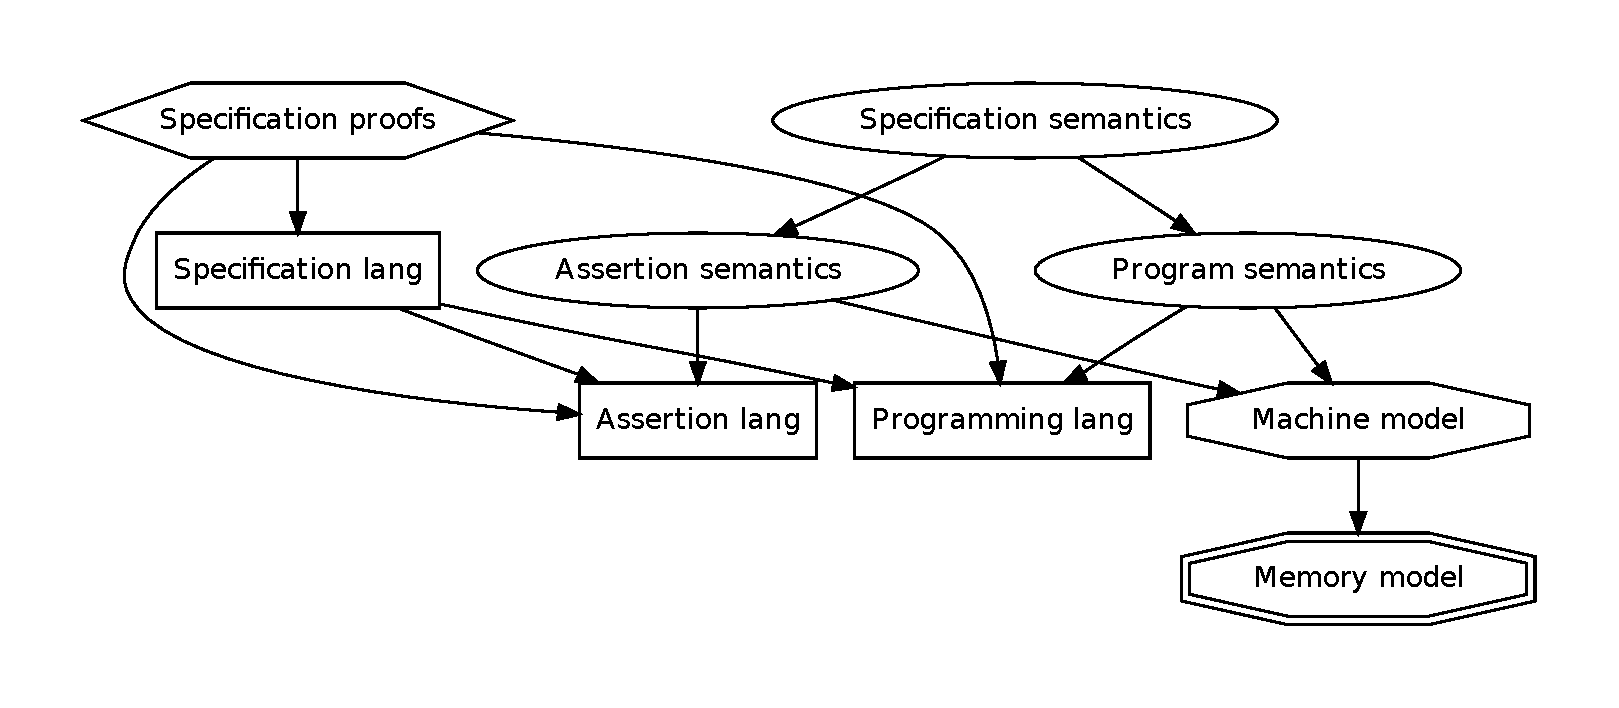
\includegraphics[scale=0.5]{dependency-graph/dg-reduced}
\caption{\label{fig:dependency-graph}Dependency graph for the project.}
\end{center}
\end{figure}

The memory model is shown in a double-lined octagon, which reflects the assumption in this project that it is complete and correct, and is not further modified from its operational definition in \cite{DBLP:conf/tphol/OwensSS09}, which is summarized in Section~\ref{sec:memory-model}. 

The machine model---in particular, the notion of machine state---depends on, but is distinct from, the memory model. For example, the memory model dictates that each processor has a private set of named registers, whereas in the machine models I shall define, a single share set of variable names is assumed. I will also take the liberty in the machine model to relax other restrictions on the notion of state from the memory model, such as the requirement that writes buffered by a single processor are totally ordered. 

The programming language is a structured C-like language with concurrent composition. It does not explicitly depend on any other components of the project. The programming language semantics relates the programming language to the machine model, and hence depends on them both. The machine models, programming language and semantics are described in Section~\ref{sec:programming-language}. 

The assertion language also does not explicitly depend on any other components of the project.\footnote{Implicitly, of course, it depends significantly on the memory and machine models.} The assertion language semantics associates the assertion language to predicates, which are defined later as sets of states (as defined by the machine model) with a particular structure. Assertions and their meaning are described in Section~\ref{sec:assertions}. 

Ideally there would also be a proof theory of assertions and a corresponding soundness theorem. I have chosen not to focus on a proof theory of assertions in this project, but will indicate some semantic implications and equivalences that would be relevant to that end in Section~\ref{sec:algebra}.

The specification language encompasses the programming and assertions languages, and its semantics is given in terms of the semantics of programs and assertions. The proof theory of specifications relies on the existence of a suitable proof theory of assertions for determining entailments. The soundness of the specification logic relies on the the soundness of the proof theory of assertions as well as the semantics of programs and assertions. Specifications are described in Section~\ref{sec:specifications}. 

\subsection{Motivation}

Why bother building a program logic? The original motivation was as follows. Although program logics are reasonable systems in which to construct hand proofs of arbitrary program properties, they have more recently been shown to be amenable to automation of relatively shallow properties, e.g., memory safety or shape properties. Unfortunately, existing logics can not be soundly applied to certain fine-grained concurrent programs like concurrent data structures. This is because these programs are typically not well locked and contain races, and so cannot rely on the underlying computer architecture to ensure that their interaction with memory is sequentially consistent. But sequential consistency is a deep assumption in most existing program logics, hence their inapplicability. 

As further motivation, concurrent data structures are inarguably important to computer science given the decline of single-threaded processor performance improvements and concomitant proliferation of parallelism. At the same time, correctness arguments for concurrent data structures are subtle enough to make informal reasoning extremely difficult. Additionally, these programs are of only modest size, which (perhaps) gives cause for optimism about their amenability to automated or semi-automated verification. Altogether, this appears to be an excellent opportunity for the application of formal methods. 

\paragraph{A Reappraisal}

I am less confident in the immediate practical value of this project than I originally was, having identified a number of errors of judgment in the original motivation. First, I was wrong to consider the small size of these programs as increasing the viability of automated reasoning about them. This is backwards: because these subtle and important programs are so small, it is entirely practical to consider hand-constructed formal proofs of their correctness using proof assistants like Coq, Isabelle or ACL2. And although constructing these proofs is difficult, surely it is less so than developing a general technique for doing so. 

Second, although such programs are clearly racy, it is not clear that their interactions with memory fall outside the bounds of sequentially consistency. And for sequentially consistent programs, it seems unlikely that an approach of such high fidelity w.r.t.~the memory model (e.g., with explicit write buffers) will turn out to be the most effective. 

Nonetheless, I still consider the project to have scientific merit. It faces the problem of local reasoning about the behavior of programs executing on a more complicated machine quite directly and gives some indication of how this can be done without relying on simplifying assumptions about memory. Local reasoning techniques can, of course, be quite useful even for hand-constructed formal proofs. 

In the best case, this work could someday provide a foundation for practically useful reasoning about a class of difficult programs. In the worst case, it sheds some light on the the problem of local program reasoning in general by providing an additional---fairly extreme---data point in the space of program logics, illustrating the difficulty and complexity of reasoning about the behavior of programs w.r.t.~a widespread and weak memory model. 

\section{Related Work}

Technical inspiration for this project comes primarily from work on separation logic \cite{DBLP:conf/lics/Reynolds02,DBLP:conf/csl/OHearnRY01,DBLP:journals/bsl/OHearnP99} and abstract separation logic \cite{DBLP:conf/lics/CalcagnoOY07}, as well as concurrent separation logic  \cite{DBLP:journals/tcs/OHearn07,DBLP:journals/tcs/Brookes07}, which this program logic resembles insofar as it strives to enable local (instead of global) reasoning about shared-state invariants (instead of two-place state relations). Although perhaps not obviously so, the semantics of the programming language was influenced by work on graphical models \cite{DBLP:journals/ipl/WehrmanHO09,DBLP:conf/RelMiCS/HoareMSW09,DBLP:journals/jlp/HoareMSW11} and the pomset model of true concurrency from Pratt \cite{DBLP:conf/popl/Pratt82,DBLP:conf/concur/Pratt84}. The style of semantics of specifications, and the associated soundness proof, is taken almost directly from Vafeiadis' recent soundness proof of concurrent separation logic \cite{V11}. Vafeiadis' excellent dissertation has also been an invaluable guide \cite{VafeiadisDissertation}. 

Also of note are two works that present solutions to the same weak-memory reasoning problem, both developed much more fully than the work I shall describe. First is Ridge's rely-guarantee program logic for the x86-TSO memory model \cite{DBLP:conf/vstte/Ridge10}. Ridge's logic is formalized in HOL and has been demonstrated with proofs of a number of interesting algorithms, including Simpsons's 4-slot non-blocking buffer. In contrast to my project, Ridge's is a logic for the x86 assembly language, whereas I target a higher level, structured language. Additionally, Ridge's logic is not inherently local, and offers nothing like the frame rule of separation logic. 

A second work of note is Cohen and Schirmer's \cite{DBLP:conf/itp/CohenS10} reduction from x86-TSO to sequential consistency for certain programs. This is notable because the class of programs they consider is larger than just the well locked programs. They show that many concurrent programming paradigms, although racy, in fact remain sequentially consistent. They furthermore provide a method of syntactic restriction for an Owicki-Gries-style program logic that allows sound reasoning about such programs. Although they describe some useful programs that fall outside of this boundary, this seems to be a work of great practical importance. Although their logic also offers no frame rule, Cohen has suggested in private communication that a similar restriction may be applied concurrent separation logic for sound local reasoning.

Related but less relevant to the current problem, compared to the previous two papers, is work by Ferreira, Feng and Shao which gives soundness proofs for concurrent separation logic in a variety relaxed-memory settings \cite{DBLP:conf/esop/FerreiraFS10}. As with the original soundness proof by Brooks \cite{DBLP:journals/tcs/Brookes07}, their theorem applies to well locked programs only, which are necessarily sequentially consistent. 

\section{Basics}

\subsection{Preliminaries and Notation}

For a set $S$ and object $o \notin S$ we write $S^o \eqdef S \uplus \set{o}$. For example, a domain $S$ can be lifted to its optional domain by writing $S^\bot$. 

\subsubsection{Functions}

For a (possibly partial) function $f : A \pfun B$ and $a \in A$ and $b \in B$, we write $\funup{f}{\ptup{a}{b}}$ for the updated function: \[ \funup{f}{\ptup{a}{b}} \eqdef \lambda x . \begin{cases}
	b & \text{if $x = a$} \\
	f(x) & \text{otherwise.}
\end{cases}\] We write $f(a) = \bot$ if the partial function $f$ is not defined at point $a$, i.e. if $a \notin \dom{f}$, and $\defined{f(a)}$ otherwise. When convenient, we also write $f_a$ as shorthand for $f(a)$. $a \mapsto b$ is shorthand for the partial function $f$ such that $f(a) = b$ and is undefined otherwise. For $A' \subseteq A$, $\restrict{f}{A'}$ is the restriction of $f$ to domain $A'$. 

For (possibly partial) functions $f,g : A \pfun B$, we we write $f \override g$ for the result of \emph{overriding} $f$ with $g$: \[ f \override g \eqdef \lambda x . \begin{cases}
	g(x) & \text{if $x \in \dom{g}$} \\
	f(x) & \text{otherwise.}
\end{cases} \] Note that if $f$ and $g$ have disjoint domains then $f \override g = f \cup g$. 

\subsubsection{Lists and Pomsets}

The empty list is denoted by $\lnil$, the singleton list by $\lsingle{o}$, and list concatenation by $l \lapp l'$, for lists $l$ and $l'$. For a list $l$ of elements drawn from a set $A \times B$, we write $\funof{l}$ for the corresponding partial lookup function: \[ \funof{l} \eqdef \lambda x .\begin{cases}
	b &\text{ if $l = l' \lapp \lsingle{(x,b)}$}\\
	\funof{l'}(x) &\text{ if $l = l' \lapp \lsingle{(y,b)}$ with $x \neq y$}\\
	\bot & \text{otherwise.}
\end{cases}\] For $A' \subseteq A$, $\restrict{l}{A'}$ is the sublist restriction of $l$ to domain $A'$.

The previous list notation is also carried over for finite pomsets: $\lnil$ for the empty pomset, $\lsingle{o}$ for the singleton pomset with label $o$, and $p \lapp p'$ for the concatenation of pomsets $p$ and $p'$. We additionally write $p \uplus p'$ for the additive union of pomsets. In contrast to the corresponding operations on partially ordered sets, these operations are total.\footnote{I assume the reader has basic familiarity with pomsets; the definition of these operations is presented nicely in \cite{DBLP:conf/icdt/GrumbachM95}.}

One subtle point is that, for $a \in A$, $\funof{p}(a)$ is defined only when there is some $b \in B$ such that $(a,b)$ is the maximum element of $p$, and undefined otherwise. Another is that, for list $l$, $\restrict{\funof{l}}{A'} = \funof{\restrict{l}{A'}}$, but, for pomset $p$, $\restrict{\funof{p}}{A'} \neq \funof{\restrict{p}{A'}}$. Consider, e.g., the two-element pomset $p = \lsingle{(a,b)} \uplus \lsingle{(a',b')}$, with $a \neq b$. Then \[\restrict{\funof{p}}{\set{a}}(a) = \bot,\] but \[\funof{\restrict{p}{\set{a}}}(a) = \funof{\lsingle{(a,b)}}(a) = b.\] 

We additionally write $p \pjoin p'$ and $p \pmeet p'$ for the partial join and partial meet of pomsets, respectively. These are intuitively are like the join and meet of partial orders, defined only when the underlying sets are equal. (The definition using pomsets is straightforward but laborious.) Given a definition of partial join, we can define a refinement partial order on pomsets in the usual way: \[ p \refines p' \iffdef p \pjoin p' = p'. \] 

When convenient, lists are treated as instances of pomsets. 

\subsection{Universes}

The various universal sets are declared and in some cases defined in Figure~\ref{fig:universes}. Note that, in the case of memory locations (i.e., addresses) and processor identifiers, 0 is excluded. 

\begin{figure}[ht]
	\centering
	\begin{tabular}{rcl|l}
		\multicolumn{3}{c}{Set} & Description \\ \hline
		\multicolumn{3}{l|}{$\setidentifiers$} & Identifiers \\
		$\setvalues$ & $=$ &  $\setintegers$ & Values \\
		$\setlocations$ & $\subseteq$  &  $\setpositives$ & Memory locations \\
		$\setprocessors$ &$\subseteq$ &  $\setpositives$ & Processor identifiers
	\end{tabular}
	\caption{\label{fig:universes}Universal Sets}
\end{figure}

\subsection{The x86-TSO Memory Model}
\label{sec:memory-model}

This section contains a brief, informal review of the x86-TSO memory model as defined by Owens, Sarkar and Sewell \cite{DBLP:conf/tphol/OwensSS09}. The model is given as a collection of legal traces of memory events. Legal traces are defined axiomatically and operationally, the latter via a labeled transition relation between machine states. These states are four-tuples $(R,m,B,l)$ in which: \begin{itemize}
	\item $R : \setprocessors \tfun \setidentifiers \pfun \setvalues$ is a register file for each processor;
	\item $m : \setlocations \pfun \setvalues$ is a shared memory; 
	\item $B : \setprocessors \tfun (\setlocations \times \setvalues)~\mathsf{list}$ is a write buffer for each processor; 
	\item $l : \setprocessors^\bot$ is a global lock. 
\end{itemize}

Transitions (labeled by memory events) between states indicate the possibility and effect of those memory events. For example, in any state $(R,m,B,l)$, processor $p$ may write a value $v$ into its register $i$; i.e., it may update the state such that $R_p(i) = v$. Similarly, if $R_p(i) = v$ then $p$ may read value $v$ from its register $i$. A summary of the other events processor $p$ may perform is as follows: \begin{itemize}
	\item it may load from its write buffer the most recent value of a location---or, if a write to that location is not found in its write buffer, from memory---if the lock is either available ($i.e.$, the lock value is $\bot$) or is held by $p$, but not if some other processor $q \neq p$ holds the lock;
	\item it may store a value to a memory location by adding a new write to the head of its write buffer regardless of the status of the lock; 
	\item it may flush (or, synonymously in this document, commit) the least recent write in its buffer to memory if it holds the lock or the lock is available;  
	\item it may fence if its buffer is empty;
	\item it may acquire the lock (i.e., change the lock value in the current state to $p$) if the lock is available; 
	\item it may release the lock (i.e., change the lock value in the current state to $\bot$) if it holds the lock.
\end{itemize}

This specification bounds the sort of memory events that can occur in program executions, but it does not give meaning to the programs of a particular language. The semantics of the programming language used in this project is however guided by the memory model, and it ought be possible to prove that it respects the bounds of the model. But this is not the focus of this project; and, even without such a correspondence proof, it will still be clear that the semantics of the programming language is manifestly weak. 

\section{The Programming Language}
\label{sec:programming-language}

In this section I describe a simplified C-like structured programming language. The primitive commands closely resemble the basic memory events described by the memory model, while the composite commands are typical for high-level languages. In particular, note that this is not assembly language. This particular language of commands was chosen to be simple to reason about, but also at a suitable level of detail for describing concurrent data structures. Such algorithms are typically expressed using high level constructs like loops and if-then-else statements, along with basic atomic constructs like compare-and-swap, indication of where fencing is required, etc. 

\subsection{Expressions and Stacks}
\label{sec:expressions}

Expressions are terms that denote values, which in this development are just integers. Hence, they are also used later on to denote memory locations and processor identifiers. 

The language of expressions, written $\exprs$, is given by the following grammar: \[ \exprs~e \bnfdef v \bnfbar x \bnfbar (e + e') \bnfbar (e - e') \bnfbar \ldots, \] where $v \in \setvalues$ and $x \in \setidentifiers$. (The possibility of additional operations is left open; the complete set of expression is not important.)

The semantics of expressions is given w.r.t.~\emph{stacks}, which are total functions from $\setidentifiers$ to $\setvalues$. The collection of functions $\setidentifiers \tfun \setvalues$ is abbreviated $\setstacks$. The interpretation of an expression w.r.t.~a stack $s$ is given by the \emph{extension} of a stack, written $\ext{s}$, which is a total function from $\exprs$ to $\setvalues$ defined as follows: \begin{align*}
	\ext{s}(v) \eqdef & v \\
	\ext{s}(x) \eqdef & s(x) \\
	\ext{s}(e + e') \eqdef & \ext{s}(e) + \ext{s}(e') \\
	\ext{s}(e - e') \eqdef & \ext{s}(e) - \ext{s}(e')
\end{align*}  

Boolean expressions are terms that denote truth values. Their language is given by the following grammar: \[ \bexprs~b \bnfdef \bexpf \bnfbar \bexpt \bnfbar (!b) \bnfbar (e = e') \bnfbar \ldots, \] where $e,e' \in \exprs$. For convenience, we represent truth values by the set $\set{0,1}$ so the extension of a stack can also be used to interpret boolean expressions: \begin{align*}
	\ext{s}(\bexpf) \eqdef & 0 \\
	\ext{s}(\bexpt) \eqdef & 1 \\
	\ext{s}(!b) \eqdef & 1 - \ext{s}(b) \\
	\ext{s}(e = e') \eqdef & \begin{cases}
		1 &\text{ if } \ext{s}(e) = \ext{s}(e')\\
		0 &\text{ otherwise.}
	\end{cases}
\end{align*}

\subsection{Commands and States}

In this setting, programs are identified with \emph{commands}, which consist of compositions of \emph{primitive commands} for accessing and modifying state. In order to restrict the scope of the project, dynamic memory management commands (e.g., memory allocation and disposal) have been omitted.\footnote{I have no particular to reason to think that they will add significant complication though, and were also considered in earlier iterations of this project \cite{wmsldetails,lola11}.}

The syntax of primitive commands is given by the following grammar: \begin{align*} \pcomms~p \bnfdef & \cskip \bnfbar \cassume{b} \bnfbar \cassert{b} \bnfbar \cassign{x}{e} \bnfbar \cload{x}{e} \bnfbar \\ 
	& \cstore{e}{e'} \bnfbar \cfence \bnfbar \clock \bnfbar \cunlock 	
\end{align*}

The informal meaning of the primitive commands is as follows. \begin{itemize}
	\item $\cskip$ takes no evaluations steps;
	\item $\cassume{b}$ evaluates to $\cskip$ if $b$ holds and becomes stuck otherwise; 
	\item $\cassert{b}$ evaluates to $\cskip$ if $b$ holds and aborts otherwise;
	\item $\cassign{x}{e}$ assigns $e$ to identifier $x$; 
	\item $\cload{x}{e}$ assigns the value at memory address $e$ to identifier $x$; 
	\item $\cstore{e}{e'}$ stores the value $e'$ to memory address $e'$; 
	\item $\cfence$ commits any buffered writes to memory; 
	\item $\clock$ acquires the global lock and fences; and
	\item $\cunlock$ releases the global lock and fences.
\end{itemize}

The formal semantics of the successful execution of a primitive command $p$ is given as a transition relation between machine states $\sigma,\sigma'$ labeled by a processor identifier $i$ \[ p \vdash \sigma \stackrel{i}{\rightarrow} \sigma'. \] An informal reading of this quadruple indicates that when $p$ is executed on processor $i$ in state $\sigma$ it may evaluate to yield state $\sigma'$. (A formal interpretation will be given later in the context of a formal semantics of full commands.) 

\begin{definition}
A partial machine state is a four-tuple $(s,h,B,k)$ such that: \begin{itemize}
	\item $s : \setidentifiers \tfun \setvalues$ is a stack, as defined in Section~\ref{sec:expressions};
	\item $h : \setlocations \pfun \setvalues$ is a \emph{heap}, i.e., a partial function that represents the allocated locations of shared memory and their values; 
	\item $B : \setprocessors \tfun (\setlocations \times \setvalues)~\mathsf{list}$ is an array of write buffers; and
	\item $k : \powerset{\setprocessors}$ is a set of blocked processors. 
\end{itemize} The collection of states is written $\setstates$. 
\end{definition}

Note that the notion of machine state given here differs from that used to define the memory model. First, the set of names (i.e., ``registers,'' ``variables,'' ``identifiers,'' etc.) are global instead of local to each processor. This is for convenience only, and is not a technical restriction. The specification logic will be restricted to programs for which the names are partitioned among processes, except for those that are never modified to. Another reasonable choice would have been to use local names only, and to share read-only values among processes in the shared memory. This has the advantage of codifying the the above healthiness condition on programs directly into the model of the language and logic; it has the disadvantage of (perhaps) describing access to shared values slightly more awkward. 

Second, the global lock value from the memory model replaced in the machine model by a set of ``blocked'' processors, which are not allowed to access main memory. In the memory model an available lock indicates that no processors are blocked, while all lock held by processor $i$ indicates that all processors but $i$ are blocked. The machine model is more general, allowing an arbitrary subset of processors to be blocked. 

A partial state is called \emph{complete} if its set of blocked processors is a valid representation of a global lock, insofar as no processors are blocked when the lock is free, and all processors but $i$ are blocked when $i$ holds the lock: \[ \complete{s,h,B,k} \iffdef k = \nil \disj \exists i \in \setprocessors \st k = \setprocessors \setminus \set{i}.\]

A primitive command may alternatively abort upon execution: \[ p \vdash \sigma \stackrel{i}{\rightarrow} \top. \] For example, an assertion may fail or a process may attempt to access an unallocated (from the process's perspective) memory address. 

As dictated by the memory model, the execution of some primitive commands is restricted by the status of the global lock. The primitive $\clock$ (resp.~$\cunlock$) can only evaluate on processor $i$ when the lock value is $\bot$ (resp.~$i$), and load can only evaluate when the lock value is either $\bot$ or $i$. There is no such restriction for store or fence, or for the other operations, which do not access the heap. 

For convenience, we define the set of \emph{live processors} w.r.t.~a given lock value as follows: \[ \live{l} \eqdef \begin{cases}
	\setprocessors &\text{ if } l = \bot\\
	\set{l} &\text{ if } l \in \setprocessors.
\end{cases}\] With this terminology, we may say that a load primitive may only evaluate on a \emph{live} processors. 

The definition of the semantic relation for primitive commands is given in Figure~\ref{fig:primitive-semantics} below. 

\begin{figure}[p]
	\centering

	\begin{minipage}{\columnwidth}

		\infrule[p-assume]{\text{ if  $\ext{s}(b) = 1$}}{\cassume{b} \vdash (s,h,B,l) \stackrel{i}{\rightarrow} (s,h,B,l)}

		\vspace{1em}

		\infrule[p-assert]{\text{ if  $\ext{s}(b) = 1$}}{\cassert{b} \vdash (s,h,B,l) \stackrel{i}{\rightarrow} (s,h,B,l)}

		\vspace{1em}

		\infrule[p-assert-a]{\text{ if  $\ext{s}(b) = 0$}}{\cassert{b} \vdash(s,h,B,l) \stackrel{i}{\rightarrow} \top}

		\vspace{1em}

		\infrule[p-assign]{}{\cassign{x}{e} \vdash(s,h,B,l) \stackrel{i}{\rightarrow} (\funup{s}{\ptup{x}{\ext{s}(e)}},h,B,l)}

		\vspace{1em}

		\infrule[p-load-b]{\text{if $\funof{B_i}(\ext{s}(e)) = v$ and $i \in \live{l}$}}{\cload{x}{e} \vdash(s,h,B,l) \stackrel{i}{\rightarrow} (\funup{s}{\ptup{x}{v}},h,B,l)}

		\vspace{1em}

		\infrule[p-load-m]{\text{if $\funof{B_i}(\ext{s}(e)) = \bot$ and $h(\ext{s}(e)) = v$ and $i \in \live{l}$}}{\cload{x}{e} \vdash(s,h,B,l) \stackrel{i}{\rightarrow} (\funup{s}{\ptup{x}{v}},h,B,l)}
		
		\vspace{1em}

		\infrule[p-load-a]{\text{if $\funof{B_i}(\ext{s}(e)) = h(\ext{s}(e)) = \bot$ and $i \in \live{l}$}}{\cload{x}{e} \vdash(s,h,B,l) \stackrel{i}{\rightarrow} \top}
		
		\vspace{1em}

		\infrule[p-store]{\text{if $\ext{s}(e) \in (\dom{\funof{B_i}} \cup \dom{h})$}}{\cstore{e}{e'} \vdash(s,h,B,l) \stackrel{i}{\rightarrow} (s,h,\funup{B}{\ptup{i}{B_i \lapp \lsingle{\ext{s}(e),\ext{s}(e')}}},l)}
		
		\vspace{1em}

		\infrule[p-store-a]{\text{if $\ext{s}(e) \notin (\dom{\funof{B_i}} \cup \dom{h})$}}{\cstore{e}{e'} \vdash(s,h,B,l) \stackrel{i}{\rightarrow} \top}
		
		\vspace{1em}

		\infrule[p-fence]{\text{if $B_i = \lnil$}}{\cfence \vdash(s,h,B,l) \stackrel{i}{\rightarrow} (s,h,B,l)}
		
		\vspace{1em}

		\infrule[p-lock]{\text{if $B_i = \lnil$}}{\clock \vdash(s,h,B,\bot) \stackrel{i}{\rightarrow} (s,h,B,i)}
		
		\vspace{1em}

		\infrule[p-unlock]{\text{if $B_i = \lnil$}}{\cunlock \vdash(s,h,B,i) \stackrel{i}{\rightarrow} (s,h,B,\bot)}
	\end{minipage}
	\caption{\label{fig:primitive-semantics} Semantics of primitive commands}
\end{figure}

Structured commands consist of either a primitive command; a sequential or concurrent composition of commands; a nondeterministic choice between commands; or an iteration of a command. We assume that, as commands, primitive commands are annotated with the name of the processor on which they are to be executed. Presumably, the components of a sequential command will all be scheduled to execute on the same processor, but this is not required and the semantics handles all cases uniformly. This generality is not likely to be practically useful for sequential composition, but is crucial to the semantics of concurrent composition, as will be discussed shortly. 

The language of commands is defined by the following grammar: \[ \comms~c \bnfdef p_e \bnfbar (\cseq{c}{c'}) \bnfbar (\cchoice{c}{c'}) \bnfbar \cloop{c} \bnfbar (\cpar{c}{c'}),\] where $p$ is a primitive command and $e$ is an expression which (hopefully) denotes a processor identifier.  

The formal semantics of the successful execution of a command is given as a binary transition relation between command-state pairs: \[ \vdash c,\sigma \rightarrow c',\sigma'.\] But a command's execution may abort unsuccessfully as well, as with primitive commands. Unsuccessful executions are modeled as a transition relation between command-state pairs and an erroneous pseudo-state, as for primitive commands: \[ \vdash c,\sigma \rightarrow \top. \] 

The semantics of commands also encompasses ``silent'' transitions, which represent the flushing of buffered writes to the shared memory as allowed by the memory model. This flushing is described by a relation between states $\stackrel{\tau}{\rightarrow}$ defined as follows: \begin{align*} (s,h,B,l) \stackrel{\tau}{\rightarrow} (s,\funup{h}{\ptup{\ell}{v}},\funup{B}{\ptup{i}{b}},l) \iffdef & B_i = \lsingle{(\ell,v)} \lapp b \conj i \in \live{l} 
\end{align*} 

The complete relation that defines the semantics of commands is given in Figure~\ref{fig:command-semantics} below.

\begin{figure}[ht]
	\centering

	\infrule[c-prim]{\text{ if $p \vdash \sigma \stackrel{\ext{s}(e)}{\rightarrow} \sigma'$ and $\sigma' \in \setstates$}}{\vdash p_e,\sigma \rightarrow \cskip,\sigma'}

	\vspace{1em}

	\begin{tabular}{ll}
	\begin{minipage}{.43\columnwidth}

		\infrule[c-prim-a]{\text{ if $p \vdash \sigma \stackrel{\ext{s}(e)}{\rightarrow} \top$}}{\vdash p_e,\sigma \rightarrow \top}

		\vspace{1em}

		\infrule[c-tau]{\text{if $\sigma \stackrel{\tau}{\rightarrow} \sigma'$}}{\vdash c,\sigma \rightarrow c,\sigma'}

		\vspace{1em}

		\infrule[c-seq]{\vdash c,\sigma \rightarrow c_0,\sigma'}{\vdash (\cseq{c}{c'}),\sigma \rightarrow (\cseq{c_0}{c'}),\sigma'}

		\vspace{1em}

		\infrule[c-seq-a]{\vdash c,\sigma \rightarrow \top}{\vdash (\cseq{c}{c'}),\sigma \rightarrow \top}

		\vspace{1em}

		\infrule[c-seq-s]{}{\vdash (\cseq{\cskip}{c'}),\sigma \rightarrow c',\sigma}

		\vspace{1em}

		\infrule[c-ch-1]{}{\vdash (\cchoice{c}{c'}),\sigma \rightarrow c,\sigma}

		\vspace{1em}

		\infrule[c-ch-2]{}{\vdash (\cchoice{c}{c'}),\sigma \rightarrow c',\sigma}

\end{minipage} & 
\begin{minipage}{.52\columnwidth}

		\infrule[c-par-1]{\vdash c,\sigma \rightarrow c_0,\sigma'}{\vdash (\cpar{c}{c'}),\sigma \rightarrow (\cpar{c_0}{c'}),\sigma'}

		\vspace{1em}

		\infrule[c-par-1a]{\vdash c,\sigma \rightarrow \top}{\vdash (\cpar{c}{c'}),\sigma \rightarrow \top}

		\vspace{1em}

		\infrule[c-par-1s]{}{\vdash (\cpar{\cskip}{c'}),\sigma \rightarrow c',\sigma}

		\vspace{1em}

		\infrule[c-par-2]{\vdash c',\sigma \rightarrow c_0,\sigma'}{\vdash (\cpar{c}{c'}),\sigma \rightarrow (\cpar{c}{c_0}),\sigma'}

		\vspace{1em}

		\infrule[c-par-2a]{\vdash c',\sigma \rightarrow \top}{\vdash (\cpar{c}{c'}),\sigma \rightarrow \top}

		\vspace{1em}

		\infrule[c-par-2s]{}{\vdash (\cpar{c}{\cskip}),\sigma \rightarrow c,\sigma}

		\vspace{1em}

		\infrule[c-loop]{}{\vdash \cloop{c},\sigma \rightarrow (\cchoice{\cskip}{(\cseq{c}{\cloop{c}})}),\sigma}

\end{minipage}
\end{tabular}
	\caption{\label{fig:command-semantics} Semantics of commands}
\end{figure} 

\paragraph{Interleaving versus Parallelism} A pleasant property of this semantics is the uniform description of both interleaving and parallel concurrency. Let $c_i$ be a sequential command $c$ in which each primitive has processor annotation $i$. Then, e.g., $(\cpar{c_1}{c'_1})$ describes the interleaving concurrent execution of commands $c$ and $c'$ on processor 1, while $(\cpar{c_1}{c'_2})$ describes the parallel concurrent execution of $c$ and $c'$ on processors 1 and 2, respectively. But one does not typically have control over the particular processor on which a command executes (e.g., $c_1$ instead of $c_2$). Thus, $(\cpar{c_x}{c'_x})$ describes the interleaving concurrent execution of commands $c$ and $c'$ on some individual processor, denoted by the free variable $x$. For $x \neq y$, $(\cpar{c_x}{c'_y})$ describes the parallel concurrent execution of $c$ and $c'$ on distinct processors given by $x$ and $y$ respectively. Furthermore, without any assumptions about the relationship between $x$ and $y$, $(\cpar{c_x}{c'_y})$ describes both interleaving and parallel executions of $c$ and $c'$. This presumably is the most common situation with concurrent composition: it is up to the operating system to assign processors to threads, and correctness of a program ought to encompass any such assignment. 
\paragraph{Abbreviations} A few standard command abbreviations are shown in Figure~\ref{fig:command-abbreviations}. Some would benefit greatly from local variable declarations, which I have not yet added to the language. 

\begin{figure}[ht]
	\centering
	\resizebox{\columnwidth}{!}{
	\begin{minipage}{\columnwidth}
	\begin{align*}
		\cifthenelse{b}{c}{c'} \eqdef & \cchoice{(\cseq{\cassume{b}}{c})}{(\cseq{\cassume{!b}}{c'})} \\
		\cifthen{b}{c} \eqdef & \cchoice{(\cseq{\cassume{b}}{c})}{(\cseq{\cassume{!b}}{\cskip})} \\
		\cwhile{b}{c} \eqdef & \cseq{\cloop{(\cseq{\cassume{b}}{c})}}{\cassume{!b}} \\
		\cwith{e}{c} \eqdef & \cseq{\clock_{e}}{\cseq{c}{\cunlock_{e}}} \\ 
		\mathsf{inc}(e,e') \eqdef & \cwith{e}{(\cseq{\cload{x}{e'}}{\cstore{e'}{x+1}})} \\
		\ccas{e,f,g,g'} \eqdef & \cwith{e}{(\cseq{\cload{x}{f}}{\cifthenelse{x = g}{\cstore{f}{g'}}{\cassign{r}{0}}})}
	\end{align*}
\end{minipage}}
	\caption{\label{fig:command-abbreviations} Command abbreviations}
\end{figure}

\paragraph{Static Semantics} The static semantics of expressions, primitive commands and commands, embodied here by functions $\fv{-}$ and $\mod{-}$ associating these objects to their sets of free and modified variables, respectively, are completely standard. (Especially so because there is are no name-hiding operations in the language, like the aforementioned missing local variable declaration command.) E.g., $\fv{\cload{x}{y+1}_z} = \set{x,y,z}$ and $\mod{\cload{x}{y+1}_z} = \set{x}$.  

\subsubsection{A More Intensional Model}

I now describe a second, different machine model and program semantics. I do this not because I believe these changes are necessary for the rest of the development, but because they have helped me in the past to understand the model and continue to make progress on the overall project. 

I refer to this second machine and program model as the ``intensional'' model, in contrast with the previous ``extensional'' model, so-called because there is some distinction between the intent of the new model (which is just the extensional model) and its denotation. In particular, the new model will use partially ordered structures to represent both the write buffers and the memory. 

The intensional model is best thought of as the composition of two changes from the extensional model: \begin{enumerate}
	\item the representation of the memory is changed from a partial function that summarizes the history of committed writes to a list that records the entire history of committed writes; and
	\item the representation of the history of writes, whether committed or buffered is relaxed from being linearly to a partially ordered. 
\end{enumerate} 

Again I emphasize that I have made these changes to provide clarity in the rest of the development, and in particular w.r.t.~later definitions of the separating conjunctions. In fact, I believe that it will \emph{not} be necessary to make pervasive use this intensional model as I am about to do in a final development of this program logic. But, because I have not yet had the opportunity to smooth out this particular wrinkle, I present it here now. 

The intensional model of state makes use of pomsets of elements drawn from $\setlocations \times \setvalues$. In particular, both the write buffers and heap are represented by pomsets. Hence, an intensional machine state is a four-tuple $(s,h,B,l)$ such that: \begin{enumerate}
	\item $s$ is a stack; 
	\item $h : (\setlocations \times \setvalues)~\mathit{pomset}$ is an intensional heap;
	\item $B : \setprocessors \rightarrow (\setlocations \times \setvalues)~\mathit{pomset}$ is an array of intensional write buffers; and 
	\item $l : \setprocessors^\bot$ is a global lock.
\end{enumerate}

The meaning of expressions is as before, but the semantics of primitive commands and commands must be revised to account for the change of machine model. Because we overload notation from lists to pomsets, the textual definition changes little. 

For the primitive commands, only load and store require modification. Informally, the changes to the semantics of primitive commands merely allow for lookups within pomsets instead of within lists (for the write buffers) and partial functions (for the heap) in the extensional semantics. For ease of reference, the complete definition of the intensional semantics of primitive commands is given in Figure~\ref{fig:int-primitive-semantics} below.

\begin{figure}[ht]
	\centering
	\resizebox{\columnwidth}{!}{
	\begin{minipage}{\columnwidth}
	\begin{align*}
		\cassume{b} \vdash & (s,h,B,l) \stackrel{i}{\rightarrow} (s,h,B,l) & \text{ if  $\ext{s}(b) = 1$} \\
		\cassert{b} \vdash & (s,h,B,l) \stackrel{i}{\rightarrow} (s,h,B,l) & \text{ if  $\ext{s}(b) = 1$} \\
		\cassert{b} \vdash & (s,h,B,l) \stackrel{i}{\rightarrow} \top & \text{ if  $\ext{s}(b) = 0$} \\
		\cassign{x}{e} \vdash & (s,h,B,l) \stackrel{i}{\rightarrow} (\funup{s}{\ptup{x}{\ext{s}(e)}},h,B,l) & \\ 
		\cload{x}{e} \vdash & (s,h,B,l) \stackrel{i}{\rightarrow} (\funup{s}{\ptup{x}{v}},h,B,l) & \text{if $\funof{\restrict{(h \lapp B_i)}{\set{\ext{s}(e)}}}(\ext{s}(e)) = v$, $i \in \live{l}$}\\ 
		\cload{x}{e} \vdash & (s,h,B,l) \stackrel{i}{\rightarrow} \top & \text{if $\restrict{(h \lapp B_i)}{\set{\ext{s}(e)}} = \lnil$, $i \in \live{l}$}\\ 
		\cstore{e}{e'} \vdash & (s,h,B,l) \stackrel{i}{\rightarrow} (s,h,\funup{B}{\ptup{i}{B_i \lapp \lsingle{\ext{s}(e),\ext{s}(e')}}},l) & \text{if $\restrict{(h \lapp B_i)}{\set{\ext{s}(e)}} \neq \lnil$} \\
		\cstore{e}{e'} \vdash & (s,h,B,l) \stackrel{i}{\rightarrow} \top & \text{if $\restrict{(h \lapp B_i)}{\set{\ext{s}(e)}} = \lnil$} \\
		\cfence \vdash & (s,h,B,l) \stackrel{i}{\rightarrow} (s,h,B,l) & \text{if $B_i = \lnil$} \\
		\clock \vdash & (s,h,B,\bot) \stackrel{i}{\rightarrow} (s,h,B,i) & \text{if $B_i = \lnil$} \\
		\cunlock \vdash & (s,h,B,i) \stackrel{i}{\rightarrow} (s,h,B,\bot) & \text{if $B_i = \lnil$}
	\end{align*}
\end{minipage}}
	\caption{\label{fig:int-primitive-semantics} Intensional semantics of primitive commands}
\end{figure}

The only substantive change between Figures~\ref{fig:primitive-semantics} and~\ref{fig:int-primitive-semantics} is that the load primitive will only  reduce to $\cskip$ when there is a unique maximum write in the state to the location under consideration. That is, if the heap is empty and $B_i = \lsingle{(\ell,v)} \lapp \lsingle{(\ell,v')}$, then $\cload{x}{\ell}$ has no transitions. This decision will be discussed shortly. 

The semantics of commands similarly requires few updates. The only substantive changes are a generalization of the $\tau$ flushing rule, and the addition of a new silent transition from less to more order-refined states. The latter is defined with the following relation on states: \[ (s,h,B,l) \stackrel{\rho}{\rightarrow} (s,h',B',l) \iffdef h' \refines h \text{ and } \forall i \in \setprocessors \st B'_i \refines B_i.\] The former is defined with the following updated relation: \begin{align*} (s,h,B,l) \stackrel{\tau}{\rightarrow} (s,h\lapp (\uplus_i B^1_i),B^2,l) \iffdef & \forall i \in \setprocessors \st B_i = B^1_i \lapp B^2_i \conj \\ & \forall i \notin \live{l} \st B^1_i = \lnil\end{align*} Whereas in the extensional semantics the oldest write of any buffer could be flushed to memory, in the intensional semantics the lower half of any directed cut of the live buffers can be flushed to memory at once, which reflects a desire to not require order among independent writes to be resolved for flushing to occur. 

The complete definition of the intensional semantics of commands is given in Figure~\ref{fig:int-command-semantics} below. 

\begin{figure}[ht]
	\centering
	\resizebox{\columnwidth}{!}{
	\begin{minipage}{\columnwidth}
	\begin{align*}
		\vdash & c,\sigma \rightarrow c,\sigma' & \text{if $\sigma \stackrel{\tau}{\rightarrow} \sigma'$} \\
		\vdash & c,\sigma \rightarrow c,\sigma' & \text{if $\sigma \stackrel{\rho}{\rightarrow} \sigma'$} \\
		\vdash & p_e,\sigma \rightarrow \cskip,\sigma' & \text{ if $p \vdash \sigma \stackrel{\ext{s}(e)}{\rightarrow} \sigma'$ and $\sigma' \in \setstates$} \\
		\vdash & p_e,\sigma \rightarrow \top & \text{ if $p \vdash \sigma \stackrel{\ext{s}(e)}{\rightarrow} \top$} \\
		\vdash & (\cseq{c}{c'}),\sigma \rightarrow (\cseq{c_0}{c'}),\sigma' & \text{ if $\vdash c,\sigma \rightarrow c_0,\sigma'$} \\
		\vdash & (\cseq{c}{c'}),\sigma \rightarrow \top & \text{ if $\vdash c,\sigma \rightarrow \top$} \\
		\vdash & (\cseq{\cskip}{c'}),\sigma \rightarrow c',\sigma & \\
		\vdash & (\cchoice{c}{c'}),\sigma \rightarrow c,\sigma & \\
		\vdash & (\cchoice{c}{c'}),\sigma \rightarrow c',\sigma & \\
		\vdash & \cloop{c},\sigma \rightarrow (\cchoice{\cskip}{(\cseq{c}{\cloop{c}})}),\sigma & \\
		\vdash & (\cpar{c}{c'}),\sigma \rightarrow (\cpar{c_0}{c'}),\sigma' & \text{ if $\vdash c,\sigma \rightarrow c_0,\sigma'$} \\
		\vdash & (\cpar{c}{c'}),\sigma \rightarrow \top & \text{ if $\vdash c,\sigma \rightarrow \top$} \\
		\vdash & (\cpar{\cskip}{c'}),\sigma \rightarrow c',\sigma & \\
		\vdash & (\cpar{c}{c'}),\sigma \rightarrow (\cpar{c}{c_0}),\sigma' & \text{ if $\vdash c',\sigma \rightarrow c_0,\sigma'$} \\
		\vdash & (\cpar{c}{c'}),\sigma \rightarrow \top & \text{ if $\vdash c',\sigma \rightarrow \top$} \\
		\vdash & (\cpar{c}{\cskip}),\sigma \rightarrow c,\sigma &
	\end{align*}
\end{minipage}}
	\caption{\label{fig:int-command-semantics} Intensional semantics of commands}
\end{figure}

We write $\refines$ for the converse of the reflexive-transitive closure of $\stackrel{\rho}{\rightarrow}$, and $\taurefines$ for converse of the reflexive-transitive closure of the union of the two relations: \[ \sigma \taurefines \sigma' \iffdef \sigma' \left( \stackrel{\tau}{\rightarrow} \cup \stackrel{\rho}{\rightarrow} \right)^{\ast} \sigma.\] 

Every step taken by $\stackrel{\rho}{\rightarrow}$ can be decomposed into two steps, one of which refines only buffered writes, and one of which refines only heap writes. We write $\sigma \stackrel{\rho_h}{\rightarrow} \sigma'$ to indicate that the buffer components of $\sigma$ and $\sigma'$ are equal (i.e., only the heap has been refined), and $\sigma \stackrel{\rho_B}{\rightarrow} \sigma'$ to indicate that the heap component of $\sigma$ and $\sigma'$ are equal (i.e., only the buffers have been refined). We refer to the former as heap refinement steps and the latter as buffer refinement steps. 

\begin{lemma}
	\label{lem:rho-decompose}
	If $\sigma \stackrel{\rho}{\rightarrow} \sigma'$ then there exists $\sigma_h$, $\sigma_B$ such that $\sigma \stackrel{\rho_h}{\rightarrow} \sigma_h \stackrel{\rho_B}{\rightarrow} \sigma'$ and $\sigma \stackrel{\rho_B}{\rightarrow} \sigma_B \stackrel{\rho_h}{\rightarrow} \sigma'$. 
\end{lemma}

Buffer refinement steps commute from right to left with $\tau$ steps, and heap refinement steps commute from left to right with $\tau$ steps. 

\begin{lemma}
	\label{lem:tau-rho-semi-commute} \hspace{1em}
	\begin{enumerate}[(i)]
		\item If $\sigma \stackrel{\tau}{\rightarrow} \sigma' \stackrel{\rho_B}{\rightarrow} \sigma''$ then there exists $\sigma_B$ such that $\sigma \stackrel{\rho_B}{\rightarrow} \sigma_B \stackrel{\tau}{\rightarrow} \sigma''$. 
		\item If $\sigma \stackrel{\rho_h}{\rightarrow} \sigma' \stackrel{\tau}{\rightarrow} \sigma''$ then there exists $\sigma_h$ such that $\sigma \stackrel{\tau}{\rightarrow} \sigma_h \stackrel{\rho_h}{\rightarrow} \sigma''$. 
	\end{enumerate}
	
\end{lemma}

\begin{lemma}
	\label{lem:rho-tau-commute}
	If $\sigma \stackrel{\rho}{\rightarrow} \sigma_\rho \stackrel{\tau}{\rightarrow} \sigma'$ then there exists $\sigma_h,\sigma_B$ such that \[ \sigma \stackrel{\rho_B}{\rightarrow} \sigma_B \stackrel{\tau}{\rightarrow} \sigma_h \stackrel{\rho_h}{\rightarrow} \sigma'.\] 
\end{lemma}

\begin{proof}
	\Calc{

		$\sigma \stackrel{\rho}{\rightarrow} \sigma_\rho \stackrel{\tau}{\rightarrow} \sigma'$

		\conn{\onlyif}{Lemma~\ref{lem:rho-decompose}}

		$\sigma \stackrel{\rho_B}{\rightarrow} \sigma_B \stackrel{\rho_h}{\rightarrow} \sigma_\rho \stackrel{\tau}{\rightarrow} \sigma'$

		\conn{\onlyif}{Lemma~\ref{lem:tau-rho-semi-commute} (ii)}

		$\sigma \stackrel{\rho_B}{\rightarrow} \sigma_B \stackrel{\tau}{\rightarrow} \sigma_h \stackrel{\rho_h}{\rightarrow} \sigma'$

	}
\end{proof}

\begin{lemma}
	\label{lem:tau-rho-commute}
	If $\sigma \stackrel{\tau}{\rightarrow} \sigma_\tau \stackrel{\rho}{\rightarrow} \sigma'$ then there exists $\sigma_h,\sigma_B$ such that \[ \sigma \stackrel{\rho_h}{\rightarrow} \sigma_h \stackrel{\tau}{\rightarrow} \sigma_B \stackrel{\rho_B}{\rightarrow} \sigma'.\] 
\end{lemma}

\begin{proof}
	\Calc{

		$\sigma \stackrel{\tau}{\rightarrow} \sigma_\tau \stackrel{\rho}{\rightarrow} \sigma'$

		\conn{\onlyif}{Lemma~\ref{lem:rho-decompose}}

		$\sigma \stackrel{\tau}{\rightarrow} \sigma_\tau \stackrel{\rho_h}{\rightarrow} \sigma_B \stackrel{\rho_B}{\rightarrow} \sigma'$

		\conn{\onlyif}{Lemma~\ref{lem:tau-rho-semi-commute} (i)}

		$\sigma \stackrel{\rho_h}{\rightarrow} \sigma_h \stackrel{\tau}{\rightarrow} \sigma_B \stackrel{\rho_B}{\rightarrow} \sigma'$

	}
\end{proof}

\begin{lemma}
	\label{lem:taurefines-decompose} $\sigma' \taurefines \sigma$ iff there exists $\sigma_B,\sigma_h$ such that $\sigma \stackrel{\rho_B}{\rightarrow} \sigma_B \stackrel{\tau}{\rightarrow} \sigma_h \stackrel{\rho_h}{\rightarrow} \sigma'$. 
\end{lemma}

\begin{proof}
	By Lemmas~\ref{lem:rho-decompose}, \ref{lem:rho-tau-commute} and~\ref{lem:tau-rho-commute}
\end{proof}

\paragraph{Why a silent refinement transition?} The silent refinement transition is needed to cope with the fact that there may be unordered writes to some location visible to a particular processor in the intensional states, but the load command can only successfully reduce when there is a unique maximum write. The silent refinement transition reduces such states until some write becomes a unique maximum. 

An ostensible alternative would be to allow the load command to return any maximal value in the state. E.g., with $B_i = \lsingle{(\ell,1)} \lapp \lsingle{(\ell,2)}$ we might allow both transitions: \begin{align*}
	\cload{x}{\ell} \vdash & (s,h,B,l) \rightarrow (\funup{s}{\ptup{x}{1}},h,B,l) \text{ and }\\ 
	\cload{x}{\ell} \vdash & (s,h,B,l) \rightarrow (\funup{s}{\ptup{x}{2}},h,B,l). 
\end{align*} But the following example shows why this definition is problematic. Consider the behavior of the following command w.r.t.~the previously defined state: \[ \cseq{\cload{x}{\ell}_i}{\cifthen{x = 1}{(\cseq{\cload{y}{\ell}_i}{\cassert{y = 1}_i})}}.\] In the intensional semantics as defined in Figures~\ref{fig:int-primitive-semantics} and~\ref{fig:int-command-semantics}, the assertion does not fail. In order for the load to have reduced, a refinement transition must first be taken in order to resolve the order between the buffered writes $(\ell,1)$ and $(\ell,2)$. The guard evaluates to 1 only when the refinement transition has resolved the order with $(\ell,1)$ above $(\ell,2)$. The following load command then must find that $1$ is the unique maximum write to location $\ell$. On the other hand, if we were to allow load to return any maximal value, then there are reduction sequences in which the first load results in $1$ and the second results in $2$, which leads to an assertion failure. Finally, note that in the extensional semantics, which is closely reflects the memory model, there also can be no assertion failure. 

\paragraph{Relating Intensional and Extensional States} There is a straightforward relationship between intensional and extensional states. As described informally at the beginning of this section, intensional states differ from extensional ones by representing the history of committed writes  instead of a summary, and by allowing partial order among the writes instead of requiring that the order be total. 

An extensional state can be converted to an intensional one by replacing the heap partial function with any list that has a lookup function equal to the former partial function. An intensional state can be converted to an extensional state by replacing each buffer pomset with a linear extension, and the heap pomset with a partial function equal to one of its linear extensions. 

These relationships can of course be made more precise, and doing so may be one path to eliminating the intensional model entirely.  

\subsection{A Concrete Model}

The model of state just presented can be thought of as an abstraction of a more concrete model of state in which the history of committed writes is recorded by the heap, instead of just the most recently committed write to each memory address. In the concrete model, both the heap and each write buffer is represented by a list of writes. The previously defined abstract states can then be seen as equivalence classes of concrete states, in which concrete states with identical stacks, locks and buffers are related iff their heaps have the same lookup function. 

As the quotient set of the concrete model, the abstract model yields relatively coarse notion of program equivalence. Conversely, a logic that is sound w.r.t.\ the concrete model is sound w.r.t.\ the abstract model as well. Given that the unified representation of shared memory and write buffers used in the concrete model leads to a dramatically simpler algebra of system specifications, we shall proceed with the concrete model. 

A \emph{concrete state} is a four-tuple $(s,h,B,l)$ such that: \begin{enumerate}
	\item $s : \setidentifiers \tfun \setvalues$ is a stack;
	\item $h : (\setlocations \times \setvalues)~\mathsf{list}$ is a concrete heap; 
	\item $B : \setprocessors \tfun ((\setlocations \times \setvalues)~\mathsf{list})$ is an array of write buffers; and 
	\item $l : \setprocessors^\bot$ is a global lock. 
\end{enumerate}  

The meaning of expressions is as before, but the semantics of primitive commands and commands must be revised to account for the change of representation of the heap. 

Among the primitive commands, only load and store require modification because only they access the heap. Informally, the changes to the semantics of primitive commands merely allow for lookups within lists instead of direct function application as in the abstract semantics. For ease of reference, the complete definition of the intensional semantics of primitive commands is given in Figure~\ref{fig:concrete-primitive-semantics} below.

\begin{figure}[p]
	\centering
	\resizebox{\columnwidth}{!}{
	\begin{minipage}{\columnwidth}

		\infrule[p-assume]{\text{ if  $\ext{s}(b) = 1$}}{\cassume{b} \vdash (s,h,B,l) \stackrel{i}{\rightarrow} (s,h,B,l)}

		\vspace{1em}

		\infrule[p-assert]{ \text{ if  $\ext{s}(b) = 1$}}{\cassert{b} \vdash (s,h,B,l) \stackrel{i}{\rightarrow} (s,h,B,l)}

		\vspace{1em}

		\infrule[p-assert-a]{\text{ if  $\ext{s}(b) = 0$}}{\cassert{b} \vdash (s,h,B,l) \stackrel{i}{\rightarrow} \top}

		\vspace{1em}

		\infrule[p-assign]{}{\cassign{x}{e} \vdash (s,h,B,l) \stackrel{i}{\rightarrow} (\funup{s}{\ptup{x}{\ext{s}(e)}},h,B,l)}

		\vspace{1em}

		\infrule[p-load]{\text{if $\funof{(h \lapp B_i)}(\ext{s}(e)) = v$ and $i \in \live{l}$}}{\cload{x}{e} \vdash (s,h,B,l) \stackrel{i}{\rightarrow} (\funup{s}{\ptup{x}{v}},h,B,l)}

		\vspace{1em}

		\infrule[p-load-a]{\text{if $\funof{(h \lapp B_i)}(\ext{s}(e)) = \bot$ and $i \in \live{l}$}}{\cload{x}{e} \vdash (s,h,B,l) \stackrel{i}{\rightarrow} \top}

		\vspace{1em}

		\infrule[p-store]{\text{if $\defined{\funof{(h \lapp B_i)}(\ext{s}(e))}$}}{\cstore{e}{e'} \vdash (s,h,B,l) \stackrel{i}{\rightarrow} (s,h,\funup{B}{\ptup{i}{B_i \lapp \lsingle{\ext{s}(e),\ext{s}(e')}}},l)}

		\vspace{1em}

		\infrule[p-store-a]{\text{if $\funof{(h \lapp B_i)}(\ext{s}(e)) = \bot$}}{\cstore{e}{e'} \vdash (s,h,B,l) \stackrel{i}{\rightarrow} \top}

		\vspace{1em}

		\infrule[p-fence]{\text{if $B_i = \lnil$}}{\cfence \vdash (s,h,B,l) \stackrel{i}{\rightarrow} (s,h,B,l)}

		\vspace{1em}

		\infrule[p-lock]{\text{if $B_i = \lnil$}}{\clock \vdash (s,h,B,\bot) \stackrel{i}{\rightarrow} (s,h,B,i)}


		\vspace{1em}

		\infrule[p-unlock]{\text{if $B_i = \lnil$}}{\cunlock \vdash (s,h,B,i) \stackrel{i}{\rightarrow} (s,h,B,\bot)}

	\end{minipage}}
	\caption{\label{fig:concrete-primitive-semantics} Concrete semantics of primitive commands}
\end{figure}

The concrete semantics of commands is defined as in Figure~\ref{fig:command-semantics}; only redefinition of the $\tau$ flushing rule is required: \begin{align*} (s,h,B,l) \stackrel{\tau}{\rightarrow} (s,h\lapp \lsingle{(\ell,v)},\funup{B}{\ptup{i}{b}},l) \iffdef & B_i = \lsingle{(\ell,v)} \lapp b \conj i \in \live{l}\end{align*} 

\section{Assertions}
\label{sec:assertions}

Assertions denote sets of machine states, and are used to write the pre- and post-conditions of commands in the specification logic. The language is defined by the following grammar: \begin{align*}
	\asserts~P \bnfdef & b \bnfbar (P \disj P') \bnfbar (P \conj P') \bnfbar (\exists x \st P) \bnfbar (\forall x \st P) \\
	& \femp \bnfbar \fbar{e} \bnfbar \flock{e,P} \bnfbar e \fwrite{e'} e'' \bnfbar \fiter{P} \bnfbar \\ 
	& (P \fhash P') \bnfbar (P \fsep P') \bnfbar (P \fseq P') \bnfbar (P \fsseq P')
\end{align*} 

The informal meaning of these assertions are as follows. The lifting of a boolean expression to an atomic formula, disjunction, conjunction and quantification have the usual meaning. $\femp$ describes states with an empty heap and all write buffers empty. $\fbar$ describes states in which just the $e$th buffer is empty. $\flock{e,P}$ changes unlocked states that satisfy $P$ to states in which processor $e$ holds the lock. $e \fwrite{e'} e''$ describes a single write to location $e$ with value $e''$, either buffer on processor $e$ or flushed to memory. $(P \fseq P')$ describes per-write buffer concatenation of writes, and $\fiter{P}$ is the Kleene closure of $P$ w.r.t.~this notion of concatenation. $(P \fsseq P')$ is like $(P \fseq P')$, but in which disjointness of allocated locations is required. $(P \fsep P')$ also requires disjointness, but interleaves the described writes on each write buffer instead of concatenating them. Finally, $(P \fhash P')$ is weaker than the three other separating conjunctions, and provides the ``most general'' frame rule. 

The set of free variables of an assertion, written $\fv{P}$, is defined as usual. 

\paragraph{Abbreviations} The following abbreviation describes the result of flushing a single write to memory: \begin{align*}
	e \fwrote e'' \eqdef & (\exists x \st e \fwrite{x} e'' \conj \fbar{x}) \\
\end{align*} (We will note later that $(e \fwrite{x} e' \conj \fbar{x})\sequiv e \fwrite{y} e' \conj \fbar{y}$, which justifies this notation.)

The Kleene closure is not necessary for expressing the axioms and inference rules of the specification logic, but is useful for defining points-to as an abbreviation. \begin{align*}
	e \fpointsto e'' \eqdef & (\exists x \st \fiter{(\exists y \st e \fwrite{x} y)} \conj \fbar{x})
\end{align*} The Kleene closure may also be useful for describing resource invariants. I have also explored other atomic formulas with more elaborate semantics for describing resource invariants, but do not bother to describe them here because of a lack of evidence for their usefulness.

\subsection{Predicates}
\label{sec:predicates}

Assertions denote particular sets of intensional machine states, which we refer to as predicates. In particular, a predicate $S$ satisfies the following three closure properties: \begin{enumerate}
	\item closure w.r.t.~flushing: if $\sigma \in S$ and $\sigma \stackrel{\tau}{\rightarrow} \sigma'$ then $\sigma' \in S$; 
	\item closure w.r.t.~refinement: if $\sigma \in S$ and $\sigma \stackrel{\rho}{\rightarrow} \sigma'$ then $\sigma' \in S$; 
	\item closure w.r.t.~partial joins: if $\sigma_1,\sigma_2 \in S$ and $\sigma_1 \pjoin \sigma_2 = \sigma'$ then $\sigma' \in S$. 
\end{enumerate} The first closure property is needed for soundness w.r.t.~the memory model. The second reflects the fact that there is no true concurrency among writes on a particular buffer, and that the partiality of ordering only represents the set of possible interleavings. The third reflects the fact that a set of possible interleavings can in turn be represented by a single partial order. Note that closure w.r.t.~partial meets is implied by the second closure property. Note also that, in an extensional model, only the first closure property is relevant. 

\subsection{Separating Conjunctions}

We now digress to define a series of functions on states, which will later be used to define the predicates for each of the four separating conjunctions. With these definitions in hand, the predicate definitions will be straightforward. 

\subsubsection{Weak Interleaving Separation}

We begin by defining a partial semantic function for the most general separating conjunction, written $\sigma \fhash \sigma'$, from which the others are derived. This operation will be particularly useful for giving meaning to program specifications, while the other, stronger conjunctions will be more useful for expressing the axioms for commands in the specification logic. 

We wish for commands to be local w.r.t.~this conjunction so that it may have a corresponding frame rule. By way of example, consider a load $\cload{x}{\ell}$ on processor $i$ in a state $\sigma$.\footnote{Ensuring locality w.r.t.~the other commands is apparently less difficult, so the exposition is focused on just load commands.} Let us consider the manners in which the state $\sigma$ can be extended while preserving the essential behavior of the command---viz.~the resultant value of the load. \begin{enumerate}
	\item We \emph{may} augment $\sigma$ with additional buffered writes to address $\ell$ on buffer $i$ if those writes occur before the most recent writes to $\ell$ on $i$. The load command only returns the most recent buffered write, so additional earlier buffered writes will not affect the result. 
	
	\item We \emph{may not} augment $\sigma$ with additional buffered writes to address $\ell$ on $i$ that are more recent than the those already present, for these additional writes certainly will affect the outcome of the load. 
	
	\item We \emph{may} augment $\sigma$ with additional committed writes to address $\ell$ if those writes again precede previously committed writes to $\ell$ in $\sigma$. (Because committed writes implicitly precede all buffered writes, this is consistent with the first scenario in which the $i$th buffer is safely augmented with earlier writes.)
	
	\item We \emph{may} augment $\sigma$ with additional writes to locations distinct from $\ell$, either committed to memory or buffered on $i$, regardless of their ordering with respect to writes to $\ell$ already present. The resultant value of the load command is not affected by writes to the locations not being loaded.  
	
	\item We \emph{may} augment $\sigma$ with additional writes to locations distinct from $\ell$ on other buffers as well. Although those writes may commit before or after the $\ell$-writes being loaded by $i$, they do not affect the result. 
	
	\item Finally, consider writes to address $\ell$ on buffers other than $i$. In general, this may adversely affect the load on $i$ because we are unable to predict the order in which these writes will commit to memory. It is possible that they will commit after buffered writes on $i$ have committed but before the load has completed, thus affecting the result of the load. So it would seem that such writes must be disallowed. 
	
	There are however cases in which it is safe to augment $\sigma$ in this way: e.g., when the lock is held by $i$. For in this case writes on other buffers will not be committed to memory, and so there is no risk that these writes will be made visible to the load on $i$. Hence, we \emph{may} augment other buffers with writes to $\ell$ when $i$ holds the lock, but we \emph{may not} when the lock is availble. 

	Furthermore, it is safe to augment the state with $\ell$-writes to other buffers when the lock is held by \emph{any} processor, and not just by $i$. For if $j$, with $j \neq i$, holds the lock, then a load on processor $i$ cannot proceed! And so, from a partial correctness standpoint, the writes on other processors are quite irrelevant.
\end{enumerate}

We now work to define a partial function on states motivated by these scenarios. We will define with what states $\sigma_0$ we may augment a given state $\sigma$, and define the result of this augmentation as $\sigma_0 \fhash \sigma$. Note that because some of the preceding scenarios are asymmetric---e.g., we may augment $\sigma$ with earlier writes to a particular location, but not later writes---the resulting operation will not be commutative. This is, of course, in contrast to the semantic function for the separating conjunction of traditional separation logic. 

We define $\sigma \fhash \sigma'$ approximately as the product of operations; one of that combines the heaps of $\sigma$ and $\sigma'$, and one that combines the individual buffers of $\sigma$ and $\sigma'$. These operations shall only constrain the order among the writes in $\sigma$ and $\sigma'$ when necessary.  Furthermore, both operations are essentially the same: the operation that combines the heaps is lifted functionally to combine the buffer arrays.

From the scenarios above, we see that the only additional ordering constraints required are between writes to the same address. Thus, the \emph{TSO union} of pomsets $p$ and $p'$, written $p \fhash p'$, is an operation that preserves the ordering among writes within $p$ and $p'$, and additionally requires, for each location $\ell$, that each write to address $\ell$ in $p$ precedes all writes to $\ell$ in $p'$. Formally, let $p = \eqclass{V,<,L,m}$ and $p' = \eqclass{V',<',L,m'}$. Then $p \fhash p'$ is defined as follows: \begin{align*}
	\eqclass{V \uplus V', < \uplus <' \uplus \setof{(v,v') \in V \times V'}{\pi_1(m(v)) = \pi_1(m'(v'))}, L, m \uplus m'},
\end{align*} where $\pi_1$ is the first projection function (i.e., $\pi_1(u,v) = u$), which in this case yields the location part of the label. We also lift this notation to functions into pomsets, e.g., write buffer arrays, in the usual way: \[ B \fhash B' \eqdef \lambda i . B_i \fhash B'_i.\]

Note that the TSO union of pomsets falls between the additive union and concatenation of pomsets in the refinement order: \[ p \lapp p' \refines p \fhash p' \refines p \uplus p'.\]  

The operation on states $\sigma \fhash \sigma'$ is partial, and much of the essence of the operation is contained in its definedness conditions. We can state the definition of the operation without discussing all of its definedness conditions, however; for now, we just note the first. Let $\sigma = (s,h,B,l)$ and $\sigma' = (s',h',B',l')$. The first definedness condition is:  \begin{align}
	s = s' \text{ and } l = l'
\end{align} Hence, we may restrict our definition of the partial operation $\sigma \fhash \sigma'$ to states $\sigma = (s,h,B,l)$ and $\sigma' = (s,h',b',l)$. The value, when defined, of $\sigma \fhash \sigma'$ is as follows: \[ (s,h,B,l) \fhash (s,h',B',l) \eqdef (s,h\fhash h',B\fhash B',l).\] 

Let us check to see whether this definition is consistent with the scenarios above: \begin{enumerate}
	\item Buffered $\ell$-writes on buffer $i$ necessarily precede any $\ell$-writes already present on buffer $i$ by definition of the TSO union of buffers, $B_i \fhash B'_i$, consistent with the corresponding scenario above. 
	
	\item Buffered writes to other locations on buffer $i$ are unordered w.r.t.~existing writes by definition of the TSO union of buffers, $B_i \fhash B'_i$, consistent with the corresponding scenario above.
	
	\item Committed $\ell$-writes necessarily precede any $\ell$-writes already present in the heap by definition of the TSO union of heaps, $h \fhash h'$, consistent with the corresponding scenario above. 
	
	\item Committed writes to other locations are unordered w.r.t.~writes already present in the heap by definition of the TSO union of heaps $h \fhash h'$, consistent with the corresponding scenario above. 
	
	\item There are no ordering constraints among buffered writes on different write buffers by definition of the TSO union of write buffer arrays, $B \fhash B'$. So in case the additional writes are to locations different from the already present writes, the definition is consistent with the corresponding scenario above. 
	
	\item Unfortunately, in the case the additional buffered writes are to locations already present on in other buffers, the definition is \emph{not} consistent with the corresponding scenario above, because $\ell$ writes may added to buffer $j$ even when $\ell$ writes already exist in buffer $i$. 
\end{enumerate}

To recover consistency, we must rule out the case in which the additional buffered writes to location $\ell$ on processor $i$ are ruled out if when writes to $\ell$ are already present in the heap, or already present in a buffer other than $i$. But, if $i$ is not live, then we need not rule out such additional writes. And we need only concern ourselves with conflicts between additional writes on $i$ and already present writes on another processor $j$ if both $i$ and $j$ are live; i.e., if the lock is available. These two conditions---ruling out conflicts among additional buffered writes with \emph{1)} the existing heap, and \emph{2)} the existing buffered writes---can be described as follows: \begin{align*}
	\forall j \in  \live{l} \st \dom{B_j} \cap \dom{h'} & = \nil \\
	\forall j \in  \live{l} \st \forall i \in \live{l} \st i \neq j \onlyif \dom{B_j} \cap \dom{B'_i} & = \nil. \\
\end{align*} Or, more succinctly, as a single condition: \[ \forall j \in \live{l} \st \dom{B_j} \cap \left( \dom{h'} \cup \bigcup_{i \in \live{l} \st i \neq j} \dom{B'_i}\right) = \nil. \] 
This, along with the requirement that the stacks and locks of the two states agree, is the definedness condition for $\sigma \fhash \sigma'$.

We refer to this as \emph{weak interleaving separation}, because only minimal ordering is created among the writes in the conjoined states (and unordered writes represent their various interleavings), and because memory addresses are not partitioned, but instead only weakly separated. 

\begin{lemma}
	\label{lem:hash-app-exchange}
	For pomsets $p,q,r,s$, $(p \fhash q) \lapp (r \fhash s) \refines (p \lapp r) \fhash (q \lapp s)$ when $\dom{q} \cap \dom{r} = \nil$. 
\end{lemma}

\begin{lemma}
	\label{lem:separation-tau}
	If $\sigma \fhash \sigma' \stackrel{\tau}{\rightarrow} \upsilon$ then there exists $\sigma_\tau,\sigma'_\tau$ such that $\sigma \stackrel{\tau}{\rightarrow} \sigma_\tau$, $\sigma' \stackrel{\tau}{\rightarrow} \sigma'_\tau$ and $\upsilon \refines \sigma_\tau \fhash \sigma'_\tau$. 
\end{lemma}

\begin{proof}
	Let $\sigma = (s,h,B,l)$ and $\sigma = (s,h',B',l)$, and so \[\sigma \fhash \sigma' = (s,h \fhash h',B \fhash B',l),\] and there exists $B_\tau^1,B_\tau^2$ such that, for all $i$, $B(i) \fhash B'(i) = B_\tau^1(i) \lapp B_\tau^2(i)$, and if $i \notin \live{l}$ then $B_\tau^1(i) = \lnil$, and \begin{align*}
		\upsilon = (s,(h \fhash h') \lapp B_\tau^1, B_\tau^2,l).
	\end{align*}

	Each of $B_\tau^1$, $B_\tau^2$ can be partitioned according to $B \fhash B'$ and rewritten as follows: \begin{align*}
		B_\tau^1 \refines & B_\tau^{1a} \fhash B_\tau^{1b} \\
		B_\tau^2 \refines & B_\tau^{2a} \fhash B_\tau^{2b}
	\end{align*} Let $\sigma_\tau = (s,h \lapp B_\tau^{1a}, B_\tau^{2a})$ and $\sigma'_\tau = (s,h' \lapp B_\tau^{1b}, B_\tau^{2b})$, and so: \begin{align*} \sigma_\tau \fhash \sigma'_\tau = (s, (h \lapp B_\tau^{1a}) \fhash (h' \lapp B_\tau^{1b}), B_\tau^{2a} \fhash B_\tau^{2b},l).
	\end{align*} To show that $\upsilon \refines \sigma_\tau \fhash \sigma'_\tau$, we must show both \begin{align*} (h \fhash h') \lapp B_\tau^1 \refines&  (h \lapp B_\tau^{1a}) \fhash (h' \lapp B_\tau^{1b}) \\ B_\tau^2 \refines&  B_\tau^{2a} \fhash B_\tau^{2b} \end{align*} The latter follows from the definition of $B_\tau^{2a}$ and $B_\tau^{2b}$. The former follows from the definition of $B_\tau^{1a}$ and $B_\tau^{2b}$ and Lemma~\ref{lem:hash-app-exchange}, using the fact that $\dom{B} \cap \dom{h'} = \nil$ and $\dom{B_\tau^{1a}} \subseteq \dom{B}$. 
\end{proof}

\begin{lemma}
	\label{lem:separation-rho-buffer}
	If $\sigma_1 \fhash \sigma_2 \stackrel{\rho_B}{\rightarrow} \sigma_B \stackrel{\tau}{\rightarrow} \sigma'$ then there exists $\sigma_{B1},\sigma_{B2}$ such that $\sigma_{1} \stackrel{\rho_B}{\rightarrow} \sigma_{B1} \stackrel{\tau}{\rightarrow} \sigma_{\tau1}$, $\sigma_{2} \stackrel{\rho_B}{\rightarrow} \sigma_{B2} \stackrel{\tau}{\rightarrow} \sigma_{\tau2}$, and $\sigma_{\tau1} \fhash \sigma_{\tau2} \stackrel{\rho}{\rightarrow} \sigma'$. 
\end{lemma}

\begin{proof}
	Here is a proof sketch. The first step involves collapsing independencies among various writes. Let $\sigma_{B1}$ be the result of collapsing those independencies among the writes of $\sigma_1$, and similarly for $\sigma_{B2}$. (This lemma does \emph{not} follow from Lemma~\ref{lem:separation-tau} because it is only the case that $\sigma_B \refines \sigma_{B1} \fhash \sigma_{B2}$, but not the other way around.) Similarly, the second step involves moving some strongly connected writes from the heap to the buffer. Let $\sigma_{\tau1}$ be the result of moving just these writes from $\sigma_{B2}$ (a fortiori, they too are strongly connected), and similarly for $\sigma_{\tau2}$. Finally, collapse independencies among the remaining writes (which may be either in the buffer or in the heap) to arrive back at $\sigma1$. 
\end{proof}

\begin{lemma}
	\label{lem:separation-refinement}
	If $\sigma \taurefines \sigma_1 \fhash \sigma_2$ then there exists $\sigma'_1,\sigma'_2$ such that $\sigma'_1 \taurefines \sigma_1$, $\sigma'_2 \taurefines \sigma_2$ and $\sigma \refines \sigma'_1 \fhash \sigma'_2$. 
\end{lemma}

\begin{proof}
	By Lemma~\ref{lem:taurefines-decompose}, there exists $\sigma_B,\sigma_h$ such that $\sigma_1 \fhash \sigma_2 \stackrel{\rho_B}{\rightarrow} \sigma_B \stackrel{\tau}{\rightarrow} \sigma_h \stackrel{\rho_h}{\rightarrow} \sigma$. By Lemma~\ref{lem:separation-refinement}, there exists $\sigma_{B1},\sigma_{\tau1},\sigma_{B2},\sigma_{\tau2}$ such that $\sigma_{1} \stackrel{\rho_B}{\rightarrow} \sigma_{B1} \stackrel{\tau}{\rightarrow} \sigma_{\tau1}$, $\sigma_{2} \stackrel{\rho_B}{\rightarrow} \sigma_{B2} \stackrel{\tau}{\rightarrow} \sigma_{\tau2}$, and $\sigma_{\tau1} \fhash \sigma_{\tau2} \stackrel{\rho}{\rightarrow} \sigma_h$. I.e., $\sigma_{\tau1} \taurefines \sigma_1$, $\sigma_{\tau2} \taurefines \sigma_2$ and $\sigma_h \refines \sigma_{\tau1} \fhash \sigma_{\tau2}$. Because $\sigma \refines \sigma_h$, we also have $\sigma \refines \sigma_{\tau1} \fhash \sigma_{\tau2}$. 
\end{proof}

It is possible to imagine strengthening this conjunction in two ways: \begin{enumerate}
	\item With stronger disjointness requirements, barring \emph{any} overlap in the addresses to which there are writes between the conjuncts, regardless of the lock status and the presence of ``covering'' writes in the present state.  
	
	\item With stronger ordering properties, yielding a state in which all writes added precede all existing writes, instead of one in which only ordering between writes to the same address is created. Weak interleaving separation is unable to express ordering constraints among writes to the same location on a single buffer. 
\end{enumerate}

The next three subsections describe separating conjunctions that embrace one or both of these additional properties. 

\subsubsection{Strong Interleaving Separation}

The strong interleaving separation of states, written $\sigma \fsep \sigma'$, is like the weak interleaving separation, but in which the domains of memory addresses are required to be completely disjoint. Later, this separation will be useful for describing the relationship between local and shared state, which we will require to be disjoint regardless of the status of the lock, and for describing concurrent composition of commands.

 The definedness condition for $\sigma \fsep \sigma$ (besides agreement on stacks and locks) is as follows: \[ \left(\dom{h} \cup \bigcup_{i \in \setprocessors} \dom{B_i} \right) \cap \left( \dom{h'} \cup \bigcup_{i \in \setprocessors} \dom{B'_i}\right) = \nil, \] and the value of $\sigma \fsep \sigma'$ is as follows: \[ (s,h,B,l) \fsep (s,h',B',l) \eqdef (s,h\fhash h',B\fhash B',l).\] 

Because the domains the heaps and buffers are disjoint, this is equivalent to the following definition that makes use of the simpler additive union in place of the TSO union: \[ (s,h,B,l) \fsep (s,h',B',l) \eqdef (s,h\uplus h',B\uplus B',l).\] 

Observe that if $\sigma \fsep \sigma'$ is defined then $\sigma \fhash \sigma'$ is defined and identical the former state. 

\subsubsection{Weak Sequential Separation}

The weak sequential separation of states, written $\sigma \fseq \sigma'$, is like the weak interleaving separation, but in which all the additional writes in $\sigma$ precede writes already present in $\sigma'$. With weak interleaving separation, the additional writes were only required to precede those already present with the same address. 

The value, when defined, of $\sigma \fseq \sigma'$ is like $\sigma \fhash \sigma'$ but uses pomset concatenation instead of the TSO union: \[ (s,h,B,l) \fseq (s,h',B',l) \eqdef (s,h \lapp h',B \lapp B',l),\] where $B \lapp B'$ is shorthand for $\lambda i . B_i \lapp B'_i$. 

We must also strengthen the definedness conditions for $\sigma \fseq \sigma'$ from that of $\sigma \fhash \sigma'$ to reflect the desire that all writes of $\sigma$ precede those of $\sigma'$. With the given definition and the definedness conditions from weak interleaving separation, the only scenario in which this condition can be violated is in the case of already present committed writes (in $h'$) conflicting with (i.e., preceding) additional buffered writes (in $B$). In the definition above, all the writes of $h \lapp h'$ implicitly precede all the writes of $B \lapp B'$, and so in particular the writes of $h'$ implicitly precede those of $B$; this is just what we rule out with the following additional definedness condition: \[ B = \nil \disj h' = \lnil \] This strong condition ensures that if any writes have committed in $\sigma'$, then $\sigma \fseq \sigma'$ is only defined if all writes have committed in $\sigma$. 

Observe that if $\sigma \fseq \sigma'$ is defined then $\sigma \fhash \sigma'$ is defined and is refined by the former state (because the concatenation of pomsets is a refinement of the TSO union of pomsets). 

\subsubsection{Strong Sequential Separation}

The strong sequential separation of states, written $\sigma \fsseq \sigma'$ combines the ideas behind the previous two notions of separation: it requires disjointness of the additional memory addresses, and also requires that all additional writes precede those already present. When defined, its value is the same as for weak sequential separation: \[ (s,h,B,l) \fsseq (s,h',B',l) \eqdef (s,h \lapp h', B \lapp B',l).\] The definedness conditions are as follows: \begin{align*}
	\left(\dom{h} \cup \bigcup_{i \in \setprocessors} \dom{B_i} \right) \cap \left( \dom{h'} \cup \bigcup_{i \in \setprocessors} \dom{B'_i}\right) & = \nil \\ 
	B = \nil \disj h' & = \lnil.
\end{align*}

Observe that if $\sigma \fsseq \sigma'$ then $\sigma \fseq \sigma'$ is defined and identical, $\sigma \fsep \sigma'$ is defined and refined by the former state, and $\sigma \fhash \sigma'$ is also defined and refined by the former state.

\subsection{Satisfaction}

The meaning of assertions is given by a satisfaction relation $\sigma \sentails P$, relating states $\sigma$ to assertions $P$. This relation is defined in two steps: first be relating some ``initial'' states to assertions, definining the \emph{kernel} of the satisfaction relation, and then closing this relation w.r.t.~refinement for the full satisfaction relation. The set of states that satisfies an assertion will be a predicate, as described in Section~\ref{sec:predicates}. 

We write $\sigma \in \presat{P}$ to indicate membership of $\sigma$ and $P$ in the kernel of the satisfaction relation, and $\presat{P}$ for the set of states related to $P$. This relation is defined by recursion on the structure of $P$ below in Figure~\ref{fig:presat-relation}. 

\begin{figure}[ht]
	\centering
	\resizebox{\columnwidth}{!}{
	\begin{minipage}{\columnwidth}
	\begin{align*}
		(s,h,B,l) \in \presat{b} \iffdef & \ext{s}(b) = 1 \\
		(s,h,B,l) \in \presat{P \disj Q} \iffdef & (s,h,B,l) \in \presat{P} \disj (s,h,B,l) \in \presat{Q} \\
		(s,h,B,l) \in \presat{P \conj Q} \iffdef & (s,h,B,l) \in \presat{P} \conj (s,h,B,l) \in \presat{Q} \\
		(s,h,B,l) \in \presat{\exists x \st P} \iffdef & \exists v \in \setvalues \st (\funup{s}{\ptup{x}{v}},h,B,l) \in \presat{P} \\
		(s,h,B,l) \in \presat{\forall x \st P} \iffdef & \forall v \in \setvalues \st (\funup{s}{\ptup{x}{v}},h,B,l) \in \presat{P} \\
		(s,h,B,l) \in \presat{\femp} \iffdef & h = \lnil \conj \forall i \in \setprocessors \st B_i = \lnil \\ 
		(s,h,B,l) \in \presat{\fbar{e}} \iffdef & \ext{s}(e) \in \setprocessors \conj B_{\ext{s}(e)} = \lnil \\ 
		(s,h,B,l) \in \presat{\flock{e,P}} \iffdef & \ext{s}(e) \in \setprocessors \conj l = \ext{s}(e) \conj (s,h,B,\bot) \in \presat{P} \\ 
		(s,h,B,l) \in \presat{e \fwrite{e'} e''} \iffdef & \ext{s}(e') \in \setprocessors \conj \\ & ((B = \ext{s}(e') \mapsto \lsingle{(\ext{s}(e),\ext{s}(e''))} \conj h = \lnil) \disj \\ 
		& \,\;(\ext{s}(e') \in \live{l} \conj B = \nil \conj h = \lsingle{(\ext{s}(e),\ext{s}(e''))})) \\
		(s,h,B,l) \in \presat{P \fhash P'} \iffdef & \exists \sigma \in \presat{P}, \sigma' \in \presat{P'} \st \sigma \fhash \sigma' = (s,h,B,l) \\
		(s,h,B,l) \in \presat{P \fsep P'} \iffdef & \exists \sigma \in \presat{P}, \sigma' \in \presat{P'} \st \sigma \fsep \sigma' = (s,h,B,l) \\
		(s,h,B,l) \in \presat{P \fseq P'} \iffdef & \exists \sigma \in \presat{P}, \sigma' \in \presat{P'} \st \sigma \fseq \sigma' = (s,h,B,l) \\
		(s,h,B,l) \in \presat{P \fsseq P'} \iffdef & \exists \sigma \in \presat{P}, \sigma' \in \presat{P'} \st \sigma \fsseq \sigma' = (s,h,B,l) \\
		(s,h,B,l) \in \presat{\fiter{P}} \iffdef & (s,h,B,l) \in \presat{\femp} \disj \\ &  \exists \sigma \in \presat{P},\sigma' \in \presat{\fiter{P}} \st (s,h,B,l) = \sigma \fseq \sigma'
	\end{align*}
\end{minipage}}
	\caption{\label{fig:presat-relation} The kernel of the satisfaction relation}
\end{figure}

The full satisfaction relation is then defined as follows: \[ \sigma \sentails P \iffdef \exists \sigma_1,\sigma_2 \in \presat{P} \st \sigma \refines (\sigma_1 \pjoin \sigma_2).\] We write $\pred{P}$ for the set of states that satisfies $P$,\[ \pred{P} \eqdef \setof{\sigma}{\sigma \sentails P},\] and also $P \sentails P'$ and $P \sequiv P'$ for semantic entailment and equivalence, respectively: \begin{align*}
	P \sentails P' \iffdef \pred{P} \subseteq \pred{P'} \\
	P \sequiv P' \iffdef \pred{P} = \pred{P'}.
\end{align*} 

\begin{lemma}
	\label{lem:separation-satisfaction}
	If $\sigma \sentails P$, $\sigma' \sentails P'$ and $\defined{\sigma \bullet \sigma'}$, then $\sigma \bullet \sigma' \sentails P \bullet P'$. 
\end{lemma}

% \begin{proof}
% 	By definition of the satisfaction relation, $\sigma \refines \sigma_1 \pjoin \sigma_2$ for some $\sigma_1,\sigma_2 \in \presat{P}$, and $\sigma' \refines \sigma'_1 \pjoin \sigma'_2$ for some $\sigma'_1,\sigma'_2 \in \presat{P'}$. By Lemma~\ref{foo}, $\sigma \bullet \sigma' \refines (\sigma_1 \bullet \sigma'_1) \pjoin (\sigma_2 \bullet \sigma'_2)$. 
% \end{proof}

\paragraph{Flushing Closure}A central claim is that, for each assertion $P$, $\pred{P}$ is a predicate; i.e., is closed w.r.t.~flushing, closed w.r.t.~refinement and closed w.r.t.~partial joins. An effect of this is that \emph{assertions are oblivious to the nondeterministic flushing of buffered writes to memory}. Intuitively, assertions may intuitively be thought to describe only the ``initial'' states, in which no nondeterministic flushing of writes has taken place, though the semantics encompasses all states reachable as a result these steps. We consider this property to be an important feature of the assertion language---and, hence, of the specification language. 

Consider, as a significant example, the set of states that satisfy the atomic formula $e \fwrite{e'} e''$. These states may be classified as follows: \begin{enumerate}
	\item states that describe a single buffered write, and 
	\item states in which that write has been committed to memory. 
\end{enumerate} Note that the lock value is unrestricted for the former states, but in the latter the lock is restricted to those processor values for which the buffer is considered live---because a write buffered on a live processor may commit nondeterministically, but a write buffered on a non-live processor may not. 

Consider as another example the states that satisfy the compound assertion $1 \fwrite{2} 3 \fseq 1 \fwrite{2} 4$. The intuitive ``initial'' state is one with two successive writes to location $1$ buffered on processor $2$. Restricting our attention to just those states in which the lock value is $\bot$, the states of the earlier left-side write assertion include ones in which the buffered write has and has not committed, and similarly for the later right-side write assertion. When these two classes states are combined with the sequential separation, three classes of states remain: those in which neither write has flushed, those in which only the earlier write has flushed, and those in which both have flushed. Crucially, the definition of weak sequential separation rules out the case in which the later write has flushed but not the earlier write. This is summarized in Figure~\ref{fig:leads-to-seq-example}. Note that this results in a set of states that is closed w.r.t.~the flushing relation. 
 
\begin{figure}[ht]
	\centering
	\resizebox{\columnwidth}{!}{
	\begin{minipage}{\columnwidth}
	\begin{tabular}{c|c|c}
		$1 \fwrite{2} 3$ &  $1 \fwrite{2} 4$ & $(1 \fwrite{2} 3) \fseq (1 \fwrite{2} 4)$\\ \hline
		$(s,\lnil,2 \mapsto \lsingle{(1,3)},\bot)$ & $(s,\lnil,2 \mapsto \lsingle{(1,4)},\bot)$ & $(s,\lnil,2 \mapsto \lsingle{(1,3)} \lapp \lsingle{(1,4)},\bot)$\\ 
		$(s,\lsingle{(1,3)},\nil,\bot)$ & $(s,\lnil,2 \mapsto \lsingle{(1,4)},\bot)$ & $(s,\lsingle{(1,3)},2 \mapsto \lsingle{(1,4)},\bot)$\\ 
		$(s,\lnil,2 \mapsto \lsingle{(1,3)},\bot)$ & $(s,\lsingle{(1,4)},\nil,\bot)$ & -- \\
		$(s,\lsingle{(1,3)},\nil,\bot)$ & $(s,\lsingle{(1,4)},\nil,\bot)$ & $(s,\lsingle{(1,3)} \lapp \lsingle{(1,4)},\nil,\bot)$\\ 
	\end{tabular}
	\end{minipage}}
	\caption{\label{fig:leads-to-seq-example}Assertion semantics example}
\end{figure}

The requirement that assertions denote sets of states that are closed w.r.t.~flushing also explains why we have chosen atomic formulas that describe empty buffers, $\fbar{e}$, as well as empty heaps and empty buffers, $\femp$. An alternative might be to use one atomic formula to describe empty heaps, say with arbitrary buffers, say $\mathbf{heapemp}$, and another to describe empty buffers with arbitrary heaps. (Then the assertion $\femp$ could be defined as a simple conjunction.) But $\mathbf{heapemp}$ is unsuitable because it does not describe a set of states that is closed under flushing. For if any write is flushed from a buffer in a state with an empty heap, the resulting state would have a heap that is nonempty. 

Also note that it is important to define the presat relation so that it preserves the flushing closure of atomic formulas, as opposed to closing the entire relation at once as with the refinement and partial-join closures.\footnote{Those closures could also be built into the presat relation, I think, but it seemed more concise to factor them out.} E.g., if $\presat{e \fwrite{i} e'}$ is not closed w.r.t.~flushing, then $\presat{\fbar{i} \conj e \fwrite{i} e'}$ is empty, and hence so too would be its flushing closure.  

\paragraph{Refinement and Partial-Join Closure}

The importance of the refinement and partial-meet closure conditions in the context of the intensional model can been seen with the following examples. Consider the following strong interleaving composition, $(x \fwrite{i} 1) \fsep (y \fwrite{i} 2)$, which consists of two unordered writes on processor $i$. The memory model is described using totally ordered write buffers, so it ought intuitively be that either the $x$ write precedes the $y$ write, or vice versa---i.e., there is no true concurrency among writes on the same buffer in the basic machine model---and so the following semantic implication ought to hold: \[ (x \fwrite{i} 1) \fsseq (y \fwrite{i} 2) \sentails (x \fwrite{i} 1) \fsep (y \fwrite{i} 2). \] This does, in fact, hold in the semantics as given because of refinement closure. Before this closure, the right-hand assertion includes only states in which the $x$ and $y$ writes are unordered. The refinement closure ensures that all linear extensions are included as well, including, e.g., the one in which the $x$ write precedes the $y$ write, as in the left-hand assertion. 

The partial-join closure, on the other hand, ensures that an assertion which denotes all possible interleavings of some writes also includes the state in which those writes are unordered. That means, in this example, that the following ought to hold as well: \[ (x \fwrite{i} 1) \fsep (y \fwrite{i} 2) \sentails ((x \fwrite{i} 1) \fsseq (y \fwrite{i} 2)) \disj ((y \fwrite{i} 2) \fsseq (x \fwrite{i} 1)). \] The partial join closure ensures this, by adding to the set of states that satisfy the right-hand assertion the join of the two states with the writes in either total order. 

Combining the previous two examples, we have the following nice semantic equivalence: \[ (x \fwrite{i} 1) \fsep (y \fwrite{i} 2) \sequiv ((x \fwrite{i} 1) \fsseq (y \fwrite{i} 2)) \disj ((y \fwrite{i} 2). \]

\subsection{Algebra}
\label{sec:algebra}

A few additional semantic equivalences and entailments are shown in Figures~\ref{fig:equivalences} and~\ref{fig:entailments}, respectively. If a formula contains instances of $\bullet$, then that is short-hand for the same formula in which the $\bullet$ has been consistently replaced by any of the four separating conjunctions. 

\begin{figure}[ht]
	\centering
	\resizebox{\columnwidth}{!}{
	\begin{minipage}{\columnwidth}
	\begin{align*}
		P  \bullet \femp \sequiv & P \\
		\femp \bullet P \sequiv & P \\
		(P \bullet P') \bullet P'' \sequiv & P \bullet (P' \bullet P'') \\
		P \fsep P' \sequiv & P' \fsep P \\
		e \fwrite{x} e' \conj \fbar{x} \sequiv & e \fwrite{y} e' \conj \fbar{y}
 	\end{align*}
	\end{minipage}}
	\caption{\label{fig:equivalences}Semantic equivalences}
\end{figure}

We note that the four separating conjunctions naturally form a sort of lattice, and that they satisfy the small exchange laws. The full exchange law only holds for the strong interleaving and sequential conjunctions. The law does not hold for the weak instantiations because, e.g., $P \fhash P'$ is not commutative. 

\begin{figure}[ht]
	\centering
	\resizebox{\columnwidth}{!}{
	\begin{minipage}{\columnwidth}
	\begin{align*}
		P \fsseq P' \sentails & P \fsep P' \\ 
		P \fsseq P' \sentails & P \fseq P' \\ 
		P \fsep P' \sentails & P \fhash P' \\ 
		P \fseq P' \sentails & P \fhash P' \\ 
		P \bullet (P' \circ P'') \sentails & (P \bullet P') \circ P'' & \text{for $P \bullet P' \sentails P \circ P'$} \\
		(P \circ P') \bullet P'' \sentails & P \circ (P' \bullet P'') & \text{for $P \bullet P' \sentails P \circ P'$} \\
		(P \fsep P') \fsseq (P'' \fsep P''') \sentails & (P \fsseq P'') \fsep (P' \fsseq P''') \\
		P \bullet P' \sentails & P'' \bullet P' & \text{if $P \sentails P''$} \\
		P \bullet P' \sentails & P \bullet P'' & \text{if $P' \sentails P''$}
 	\end{align*}
 	\end{minipage}}
	\caption{\label{fig:entailments}Semantic entailments}
\end{figure}


\section{Specifications}
\label{sec:specifications}

The language of specifications is given by the following schema: \[ \spec{J}{P}{c}{Q}, \] where $c$ is a command and $J,P,Q$ are assertions, referred to as the \emph{invariant}, \emph{precondition} and \emph{postcondition}, respectively. 

\subsection{Semantics}

A specification asserts the partial correctness of a command. Their informal meaning is roughly analogous to that of concurrent separation logic: if $c$ is evaluated in a state that satisfies $J \fsep P$, then: \emph{1)} it does not abort, \emph{2)} it maintains the invariant $J$ during execution, and \emph{3)} if it evaluates fully, it terminates in a state that satisfies $J \fsep Q$. 

Following Vafeiadis \cite{V11}, the formal semantics of specifications is given by a family of predicates, $\safe{n}{c,\sigma,J,Q}$, parametrized by $n \in \setnaturals$, that relate a command $c$, state $\sigma$, invariant assertion $J$ and postcondition $Q$ according to the informal explanation above. Once these predicates are defined, we define truth of specifications as follows: \[ \truespec{J}{P}{c}{Q} \iffdef \forall \sigma \sentails P \st \forall n \in \setnaturals \st \safe{n}{c,\sigma,J,Q}.\]

In the sequel, let $\locked{\sigma}$ indicate that some processor holds the lock state $\sigma$: \[ \locked{s,h,B,l} \iffdef l \in \setprocessors. \]

We now give a formal definition of $\safe{n}{c,\sigma,J,Q}$ by natural number induction on $n$. $\safe{0}{c,\sigma,J,Q}$ holds always. And for $n \in \setnaturals$, $\safe{n+1}{c,\sigma,J,Q}$ holds iff the following conditions are true: \begin{enumerate}
	\item If $c = \cskip$ then $\sigma \in Q$

	\item For all $\sigma_J,\sigma_F$ such that \begin{enumerate}[(i)]
		\item $\defined{\sigma_J \fsep (\sigma_F \fhash \sigma)}$, and 
		\item either $\sigma_J \sentails J$ or $\locked{\sigma_J}$,
	\end{enumerate} $c,(\sigma_J \fsep (\sigma_F \fhash \sigma)) \nrightarrow \top$

	\item For all $\sigma_J,\sigma_F,\sigma_1,c'$ such that \begin{enumerate}[(i)]
		\item $\defined{\sigma_J \fsep (\sigma_F \fhash \sigma)}$,
		\item either $\sigma_J \sentails J$ or $\locked{\sigma_J}$, and 
		\item $c, (\sigma_J \fsep (\sigma_F \fhash \sigma)) \rightarrow c',\sigma_1$,
	\end{enumerate} there exists $\sigma'_J,\sigma'_F,\sigma'$ such that \begin{enumerate}
		\item $\sigma_1 \refines \sigma'_J \fsep (\sigma'_F \fhash \sigma')$,
		\item $\sigma'_F \taurefines \sigma_F$,
		\item either $\sigma'_J \sentails J$ or $\locked{\sigma'_J}$, and
		\item $\safe{n}{c',\sigma',J,Q}$.
	\end{enumerate}

\end{enumerate}

The definition of the predicate above differs from Vafeiadis' in three ways. First, the separating conjunctions are obviously different and, in particular, there are two different separating conjunctions used: one for framing and one for partitioning the local from the shared state. It may be possible (or even necessary) to make use of $\fhash$ uniformly in the definition, which would yield a stronger notion of specification.\footnote{Checking this specifically is next on my agenda. I have in the past proved the soundness of the frame rules with semantics similar to, but not identical to, the one presented.} Second, the frame state is allowed to change from one step to another, but only by making silent transitions. Third, because there is no inherent notion of atomicity, we cannot require that the system state always be separable so that one part satisfies the invariant assertion. For even while one processor holds the lock, others may continue to execute. Hence, we weaken the invariant condition to require only that it hold while the lock is available.

\subsection{Proof Theory}

The axioms of the logic are given in Figure~\ref{fig:axioms}.

\begin{figure}[ht]
	\centering
	\resizebox{\columnwidth}{!}{
	\begin{minipage}{\columnwidth}
		\infax[skip]{\spec{J}{P}{\cskip_i}{P}} 
		\vspace{1em}
		
		\infax[assume]{\spec{J}{!b \disj P}{\cassume{b}_i}{P}}
		\vspace{1em}
		
		\infax[assert]{\spec{J}{b \conj P}{\cassert{b}_i}{P}}
		\vspace{1em}
		
		\infax[assign]{\spec{J}{P\subst{e}{x}}{\cassign{x}{e}_i}{P}}
		\vspace{1em}
		
		\infax[load-buf]{\spec{J}{(e \fwrite{i} e') \fsseq P}{\cload{x}{e}_i}{((e \fwrite{i} e') \fsseq P)\conj x = e'}}
		\vspace{1em}
		
		\infax[load-mem]{\spec{J}{(e \fwrote e') \fsseq P}{\cload{x}{e}_i}{((e \fwrote e') \fsseq P) \conj x = e'}}
		\vspace{1em}
		
		\infax[store]{\spec{J}{(e \fwrote e'') \fseq P}{\cstore{e}{e'}_i}{(e 
		\fwrote e'') \fseq P \fseq (e \fwrite{i} e')}}
		\vspace{1em}
		
		\infax[fence]{\spec{J}{P}{\cfence_i}{P \conj \fbar{i}}}
		\vspace{1em}
		
		\infax[lock]{\spec{J}{P}{\clock_i}{\flock{i,P} \conj \fbar{i}}}
		\vspace{1em}
		
		\infax[unlock]{\spec{J}{\flock{i,P}}{\cunlock_i}{P \conj \fbar{i}}}
	\end{minipage}}
	\caption{\label{fig:axioms}Axioms}
\end{figure}

The axioms for $\cskip$, $\cassume{b}$, $\cassert{b}$ and $\cassign{x}{e}$ are as usual. The two axioms for $\cload{x}{e}$ reflect the fact that the write to be loaded may reside either in the buffer or in the heap. The schematic variable $P$ may be used to describe buffered writes to locations other than $e$ that are more recent than the write to $e$ being loaded, but not more recent writes to $e$. 

The write in the precondition of the store axiom is a witness to the allocation status of $e$. There are other possible axioms for the store command, e.g.: 
	\infax[store-buf]{\spec{J}{(e \fwrite{i} e'') \fsseq P}{\cstore{e}{e'}_i}{((e \fwrite{i} e'') \fsseq P) \fseq e \fwrite{i} e'}}

	\infax[store-mem]{\spec{J}{(e \fwrote e'') \fsseq P}{\cstore{e}{e'}_i}{((e \fwrote e'') \fsseq P) \fseq e \fwrite{i} e'}}
These reflect the two cases distinguished by the load axioms, and may or may not be more useful in practice. The axiom for $\cfence$ simply filters away states in which there are buffered writes. The axioms for $\clock$ and $\cunlock$ reflect the fact those commands are associated with implicit fences.

The logical and structural inference rules of the logic are given in Figures~\ref{fig:logical-inference-rules} and~\ref{fig:structural-inference-rules}, respectively.

\begin{figure}[ht]
	\centering
	\resizebox{\columnwidth}{!}{
	\begin{minipage}{\columnwidth}

		\infrule[disj]{\spec{J}{P}{c}{Q} \text{~~~} \spec{J}{P'}{c}{Q}}{\spec{J}{P \disj P'}{c}{Q}}
		\vspace{1em}

		\infrule[ex]{\spec{J}{P}{c}{Q} \text{~~~} x \notin \fv{c,P}}{\spec{J}{\exists x \st P}{c}{Q}}
		\vspace{1em}

		\infrule[frame-wi]{\spec{J}{P}{c}{Q} \text{~~~} \mod{c} \cap \fv{R} = \nil}{\spec{J}{R \fhash P}{c}{R \fhash Q}}
		\vspace{1em}

		\infrule[frame-si]{\spec{J}{P}{c}{Q} \text{~~~} \mod{c} \cap \fv{R} = \nil}{\spec{J}{R \fsep P}{c}{R \fsep Q}}
		\vspace{1em}

		\infrule[frame-ws]{\spec{J}{P}{c}{Q} \text{~~~} \mod{c} \cap \fv{R} = \nil}{\spec{J}{R \fseq P}{c}{R \fseq Q}}
		\vspace{1em}

		\infrule[frame-ss]{\spec{J}{P}{c}{Q} \text{~~~} \mod{c} \cap \fv{R} = \nil}{\spec{J}{R \fsseq P}{c}{R \fsseq Q}}
		\vspace{1em}

		\infrule[cons]{P \sentails P' \text{~~~}\spec{J}{P'}{c}{Q'} \text{~~~} Q' \sentails Q}{\spec{J}{P}{c}{Q}}

	\end{minipage}}
	\caption{\label{fig:logical-inference-rules}Logical inference rules}
\end{figure}

The logical rules require little explanation. Observe that there is a single left-side frame rule for each of the four separating conjunctions. The strong interleaving conjunction is commutative, and so with the rule of consequence effectively provides a right-side frame rule as well. 

There has been no attempt to provide a conjunction rule because there has been no attempt as yet to identify a suitable notion of precision~\cite{DBLP:journals/entcs/GotsmanBC11}. 

\begin{figure}[ht]
	\centering
	\resizebox{\columnwidth}{!}{
	\begin{minipage}{\columnwidth}

		\infrule[seq]{\spec{J}{P}{c}{R} \text{~~~} \spec{J}{R}{c'}{Q}}{\spec{J}{P}{\cseq{c}{c'}}{Q}}
		\vspace{1em}

		\infrule[choice]{\spec{J}{P}{c}{Q} \text{~~~} \spec{J}{P}{c'}{Q}}{\spec{J}{P}{\cchoice{c}{c'}}{Q}}
		\vspace{1em}

		\infrule[loop]{\spec{J}{P}{c}{P}}{\spec{J}{P}{\cloop{c}}{P}}
		\vspace{1em}

		\infrule[inv]{\spec{\femp}{J \fsep \flock{i,P}}{c}{J \fsep \flock{i,Q}}}{\spec{J}{\flock{i,P}}{c}{\flock{i,Q}}}
		\vspace{1em}

	 	\infrule[conc]{\spec{J}{P}{c}{Q} \text{~~~}\spec{J}{P'}{c'}{Q'} \text{~~~} \fv{P,c,Q} \cap \mod{c'} = \nil \text{, etc.}}{\spec{J}{P \fsep P'}{\cpar{c}{c'}}{Q \fsep Q'}}


	\end{minipage}}
	\caption{\label{fig:structural-inference-rules}Structural inference rules}
\end{figure}

The structural rules for sequential composition, nondeterministic choice, loops and concurrency are as in Concurrent Separation Logic. In particular, the concurrency rule requires agreement between the two processes on the value shared invariant, and the strong interleaving separating conjunction is used to partition the local states. Note that both this conjunction and the concurrent composition command are commutative. Only the invariant rule differs from Concurrent Separation Logic. There, we require that the lock be held while accessing the shared invariant. 

Using the invariant rule and the axioms for $\clock$ and $\cunlock$, we can derive the following rule for reasoning about ``locked'' commands implemented on x86, like atomic increment or compare-and-swap: \infrule[locked]{\spec{\femp}{J \fsep \flock{i,P} \conj \fbar{i}}{c}{J \fsep \flock{i,Q}}}{\spec{J}{P}{\cseq{\clock_i}{\cseq{c}{\cunlock_i}}}{Q \conj \fbar{i}}}

\begin{figure}[ht]
	\centering
	\resizebox{\columnwidth}{!}{
	\begin{minipage}{\columnwidth}

		\infrule[shared-load]{\spec{\femp}{J \fsep P}{\cload{x}{e}_i}{J \fsep Q}}{\spec{J}{P}{\cload{x}{e}_i}{Q}}
		\vspace{1em}

		\infrule[shared-store]{\spec{\femp}{J \fsep P}{\cstore{e}{e'}_i}{J \fsep Q}}{\spec{J}{P}{\cstore{e}{e'}_i}{Q}}

	\end{minipage}}
	\caption{\label{fig:daring-structural-inference-rules}Daring structural inference rules}
\end{figure} 

Figure~\ref{fig:daring-structural-inference-rules} shows two additional ``daring'' inference rules, the soundness of which may well be quite difficult to demonstrate. These rules differ from the invariant rule because they allow reasoning about the behavior of individual load and store instructions in which the value of the lock is unspecified. Intuitively, the shared load rule might be shown to be true because a load may only proceed on a live processor, and so will never access shared state while it is being modified by another process, which holds the lock. On the other hand, the shared store axiom might be shown to be true because although a store may take place while another process is modifying the shared state---and hence while the shared state does not satisfy the stated invariant $J$---the buffered write will not commit until the other process has released the lock and repaired the shared state, restoring the invariant.

The daring rules may be needed to reason about, e.g., x86 spinlock implementations. The spinlock is typically acquired using a compare-and-swap instruction, which in this language is simply a locked if-the-else command. The invariant rule and lock axioms thus should be sufficient for demonstrating correctness of spinlock acquisition. But the spinlock is released by writing to a shared memory address without first acquiring the global lock or fencing. This obviates the invariant rule, but not the shared write rule, and so there is yet hope. 

\subsection{Soundness}

\begin{lemma}
	\label{lem:weak-interleaving-safe}
	If $\safe{n}{c,\sigma,J,Q}$, $\fv{R} \cap \mod{c} = \nil$, $\defined{\sigma_R \fhash \sigma}$, and $\sigma_R \sentails R$, then $\safe{n}{c, \sigma_R \fhash \sigma,J,R \fhash Q}$. 
\end{lemma}

\begin{proof}
	By induction on $n$. The base case is trivial. For the induction step, we assume the lemma holds for $n$ and show that it holds for $n+1$. That is, we assume, for any $c,\sigma,\sigma_R,J,Q,R$, that whenever $\safe{n}{c,\sigma,J,Q}$, $\fv{R} \cap \mod{c} = \nil$, $\defined{\sigma_R \fhash \sigma}$, and $\sigma_R \sentails R$, it is also the case that $\safe{n}{c,\sigma_R \fhash \sigma,J,R \fhash Q}$ holds. We also assume that $\safe{n+1}{c,\sigma,J,Q}$, $\fv{R} \cap \mod{c} = \nil$, $\defined{\sigma_R \fhash \sigma}$, and $\sigma_R \sentails R$, and show that \\ 
	$\safe{n+1}{c,\sigma_R \fhash \sigma,J,R \fhash Q}$. To show this, we must establish three conditions. 

	\begin{enumerate}
		\item Suppose $c = \cskip$. By assumption, $\sigma_R \sentails R$, $\defined{\sigma_R \fhash \sigma}$, and if $c = \cskip$ then $\sigma \sentails Q$, and so $\sigma \sentails Q$. By Lemma~\ref{lem:separation-satisfaction}, $\sigma_R \fhash \sigma \sentails R \fhash Q$. 

		\item Let $\sigma_J,\sigma_F$ such that $\defined{\sigma_J \fsep (\sigma_F \fhash (\sigma_R \fhash \sigma))}$, and either $\locked{\sigma_J}$ or $\sigma_J \sentails J$. We must show that $\sigma_J \fsep (\sigma_F \fhash (\sigma_R \fhash \sigma)) \nrightarrow \top$. But \[ \sigma_J \fsep (\sigma_F \fhash (\sigma_R \fhash \sigma)) = \sigma_J \fsep ((\sigma_F \fhash \sigma_R) \fhash \sigma),\] and so by part 2 of assumption $\safe{n+1}{c,\sigma,J,Q}$, instantiating with $\sigma_F \fhash \sigma_R$, the result holds. 

		\item Let $\sigma_J,\sigma_F,\sigma_1,c'$ such that $\defined{\sigma_J \fsep (\sigma_F \fhash (\sigma_R \fhash \sigma))}$, either $\locked{\sigma_J}$ or $\sigma_J \sentails J$, and $c,(\sigma_J \fsep (\sigma_F \fhash (\sigma_R \fhash \sigma))) \rightarrow c',\sigma_1$. We must exhibit $\sigma'_J,\sigma'_F,\sigma'$ such that: \begin{enumerate}[(a)]
			\item $\sigma_1 \refines \sigma'_J \fsep (\sigma'_F \fhash \sigma')$,
			\item $\sigma'_F \taurefines \sigma_F$, 
			\item either $\locked{\sigma'_J}$ or $\sigma'_J \sentails J$, and
			\item $\safe{n}{c',\sigma',J,R \fhash Q}$. 
		\end{enumerate}

		We instantiate part 3 of assumption $\safe{n+1}{c,\sigma,J,Q}$ with $\sigma_J$, $\sigma_F \fhash \sigma_R$, $\sigma_1$ and $c'$, which gives us $\sigma'_J, \sigma'_{FR}, \sigma'$ such that: \begin{enumerate}[(a)]
			\item $\sigma_1 \refines \sigma'_J \fsep (\sigma'_{FR} \fhash \sigma')$
			\item $\sigma'_{FR} \taurefines \sigma_F \fhash \sigma_R$
			\item either $\locked{\sigma'_J}$ or $\sigma'_J \sentails J$, and
			\item $\safe{n}{c',\sigma',J,Q}$.
		\end{enumerate}	

		By Lemma~\ref{lem:separation-refinement} and $\sigma'_{FR} \taurefines \sigma_F \fhash \sigma_R$, there exists $\sigma'_F,\sigma'_R$ such that $\sigma'_F \taurefines \sigma_F$, $\sigma'_R \taurefines \sigma_R$ and $\sigma'_{FR} \refines \sigma'_F \fhash \sigma'_R$. 

		From $\sigma'_R \taurefines \sigma_R$ and $\sigma_R \sentails R$, it follows that $\sigma'_R \sentails R$. 

		Next, we wish to apply the inductive hypothesis to $\safe{n}{c',\sigma',J,Q}$ to show that $\safe{n}{c',\sigma'_R \fhash \sigma',J,R \fhash Q}$. This follows from the observations that $\fv{R} \cap \mod{c'} = \nil$ (because $\mod{c'} \subseteq \mod{c}$) and $\defined{\sigma'_R \fhash \sigma'}$. 

		Returning to our original task, we exhibit $\sigma'_J$, $\sigma'_F$ and $\sigma'_R \fhash \sigma'$. By associativity and monotonicity it follows that \[ \sigma_1 \refines \sigma'_J \fsep (\sigma'_F \fhash (\sigma'_R \fhash \sigma')).\] We already showed that $\sigma'_F \taurefines \sigma_F$. Either $\locked{\sigma'_J}$ or $\sigma'_J \sentails J$ by assumption. Finally $\safe{n}{c',\sigma'_R \fhash \sigma',J,R \fhash Q}$ by the inductive hypothesis above. 

	\end{enumerate}
\end{proof}

\begin{lemma}[Weak Interleaving Frame Soundness]
	If $\truespec{J}{P}{c}{Q}$ and $\fv{R} \cap \mod{c} = \nil$ then $\truespec{J}{R \fhash P}{c}{R \fhash Q}$. 
\end{lemma}

\begin{proof}
	Let $\sigma \sentails R \fhash P$ and $n \in \setnaturals$. We must show $\safe{n}{c,\sigma,J,R\fhash Q}$. From $\sigma \sentails R \fhash P$, there exists $\sigma_R \sentails R$ and $\sigma_P \sentails P$ with $\defined{\sigma_R \fhash \sigma_P}$. By assumption, $\safe{n}{c,\sigma_P,J,Q}$. The result follows from Lemma~\ref{lem:weak-interleaving-safe}. 
\end{proof}

\section{Outlook}

It remains to show soundness of the proof theory of specifications, i.e., that \[ \spec{J}{P}{c}{Q} \text{ is provable only when } \truespec{J}{P}{c}{Q}\] Some aspects of this development concern me more than others in regard to this task. 

I am confident in the programming language semantics, and (as mentioned earlier), believe that ultimately only the extensional semantics will be needed. There are many questions to be answered about the relationship between the intensional semantics and the extensional one, but I believe this is less important than exploring soundness of specification logic. I am also fairly confident in the definitions of the separating conjunctions--- in spirit, at least, and w.r.t.~the given model of state---and believe the semantic implications and equivalences stated will be completely straightforward to show. 

On the other hand, the $\flock{e,P}$ assertion and the rules for manipulating it have only recently been developed, and so problems there are likely. I am still exploring other options for defining $\flock{e,P}$, including a more ``multiplicative'' definition. And although I am not aware of any particular problems with the ``additive'' definition of $\fbar{e}$, that too has a comparatively fresh definition and could well cause problems. The treatment of the invariant and the lock in the definition of the \textsf{safe} predicate gives me pause; yet for the moment I see no other suitable definition. The axioms for load and store are, I believe, sound, but it is unclear whether a different assertion language would yield more general axioms. I would also not be surprised to find it necessary to abandon the small axioms for the $\clock$ and $\cunlock$ commands and the general invariant rule in favor of a more restricted rule in line with the derived rule for locked commands. 

In any case, I expect that something will have changed by the time you have finished reading this document, and that that change is cascading through the rest of the development, yielding new insights and necessitating additional changes, and so on, and so forth.  

\bibliography{dissertation}
\bibliographystyle{abbrv} 

\end{document} 
